\documentclass[a4paper, 12pt] {report}
\renewcommand{\baselinestretch}{1.5}

\usepackage[utf8]{inputenc}
\usepackage[italian]{babel}
\usepackage[T1]{fontenc}
\usepackage[margin=2.5cm, lmargin=3.5cm]{geometry}
\usepackage{float}
\usepackage{graphicx}
\usepackage[rightcaption]{sidecap}
\usepackage[font=footnotesize, labelfont=bf]{caption}
\usepackage[sorting=none]{biblatex}
\usepackage{listings}
\usepackage[toc,page]{appendix}
\usepackage{soul}
\usepackage{courier}
\usepackage{lettrine}
\usepackage{csquotes}
\usepackage{eurosym}
\usepackage{pifont}
\usepackage{url}
\usepackage{hyperref}
\usepackage{frontespizio}

\addbibresource{ref.bib}

\title{Sincronizzazione dei dati tramite protocolli HTTP e MQTT}
\author{Francesco Carnielli}
\date{}
\makeindex

\begin{document}

  \begin{frontespizio}
    \Margini{3.5cm}{2.5cm}{2.5cm}{2.5cm}
    \Universita{Verona}
    \Facolta{Scienze Matematiche, Fisiche e Naturali}
    \Corso[Laurea Triennale]{Informatica}
    \Annoaccademico{2016--2017}
    \Titolo{Sincronizzazione dei dati tramite protocolli HTTP e MQTT}
    \Candidato[VR087968]{Francesco Carnielli}
    \Relatore{Prof. Damiano Carra}
    \Correlatore{Prof. X X}
  \end{frontespizio}

  % remove pagenumber from here
  \pagenumbering{gobble}

  \newpage
  \thispagestyle{empty}
  \mbox{}

  \clearpage
  \pagenumbering{Roman}
  \setcounter{page}{1}

  \begin{abstract}
    Scopo del lavoro di questa tesi è individuare ed analizzare i protocolli di rete in grado di mantenere i dati sincronizzati tra client e server.
A seguito di un evento, gli interlocutori devono essere avvisati in tempo utile, ottimizzando le risorse disponibili ed aggiornando le eventuali risorse.

Nel dettaglio si analizzeranno i protocolli HTTP e MQTT, la loro evoluzione, progettazione e gli scenari d'uso.
Verranno presentati due applicativi sviluppati presso Supermercato24, i requisiti iniziali, la loro risoluzione e le scelte tecniche intraprese.

Infine si valuteranno, tramite benchmark, la bontà di questi protocolli con i loro pro e contro, illustrando possibili conseguenze future.

  \end{abstract}

  \chapter*{Ringraziamenti}
    \label{ch:acknowledgements}
    Il lavoro di tesi svolto e presentato in questo elaborato non avrebbe mai potuto essere portato avanti e finito senza il supporto di tutte quelle persone che hanno dedicato parte del loro tempo e delle loro energie per aiutarmi e per ascoltarmi.

In primo luogo vorrei ringraziare tutti i ragazzi di Supermercato24, in particolar modo Marco Risi, che in questi due anni di lavoro diurno e notturno l'hanno resa l'azienda che è oggi.

Ringrazio di cuore tutti gli amici della mia compagnia per avermi costantemente spronato e sostenuto.

Ringrazio infine la mia famiglia per il sostegno fornito in questi anni.


  \newpage
  \thispagestyle{empty}
  \mbox{}

  \tableofcontents

  \newpage
  \thispagestyle{empty}
  \mbox{}

  % starting pagenumber from here
  \clearpage
  \pagenumbering{arabic}
  \setcounter{page}{1}

  \chapter{Introduzione}
    \label{ch:intro}
    \lettrine{I}{nternet} e le tecnologie informatiche digitali più generali, hanno permesso un'ampia base di cambiamenti nell'organizzazione delle attività economiche così profonde da giustificare il titolo di rivoluzione, definita sotto l'aspetto tecnologico e socio-culturale.
L'informazione può essere più facilmente collezionata, salvata, processata, resa disponibile, comunicata ed utilizzata.
La riduzione del costo di comunicazione comporterà un aumento del traffico, maggior accesso alle informazioni, autonomia personale nella scelta delle decisioni ed ultimamente nella dispersione delle attività economiche \cite{InternetRevolution}.

Di riflesso, i protocolli e le strutture con cui queste interconnessioni vengono stabilite stanno subendo un'incessante evoluzione, mantenendo la rete accessibile a tutti come mezzo libero di informazione e comunicazione.
La costante necessità di avere tutte le informazioni immediatamente disponibili, tempestivamente aggiornate ed il rapido aumento dei dispositivi connessi, che sono sia consumatori sia produttori di dati, richiede diversi approcci per adeguarsi a queste nuove esigenze.
Il traffico dati generato si raddoppia approssimativamente ogni anno. Questo dato rappresenta una crescita estremamente rapida, maggiore di qualsiasi altro servizio di comunicazione.
Se la mole di informazioni transitata su Internet continua a raddoppiare ogni anno, potrebbe essere necessaria un'altra forma della \textit{Legge di Moore} \cite{Moore}.

Mantenere i dati sincronizzati attraverso diversi dispositivi connessi è diventato un pattern comune tra tutti i moderni software con funzionalità di rete.
Ogni utente si aspetta, come \verb+UX+ (\textit{User Experience}), di aprire la propria casella di posta con il cellulare e vedere le stesse e-mail viste precedentemente su desktop. Alla ricezione di una nuova e-mail, dovrà ricevere il giusto avviso sui propri dispositivi.
In un servizio di messaggistica istantanea, ci si aspetta di ricevere un messaggio il più velocemente possibile e non al prossimo caricamento dell'interfaccia.
Modificando un file condiviso, questo deve essere aggiornato necessariamente con le ultime modifiche, per evitare di lavorare su una revisione già obsoleta.
Con l'eterogeneità dei dispositivi e la ricerca di standard comuni, questo paradigma può non sembrare così semplice.
La crescente mole di dati rappresenta un problema per le strutture sottostanti.
Perciò diventa fondamentale trovare il giusto compromesso tra le richieste di design e la stabilità dell'implementazione.

In questo elaborato verranno descritti i principali protocolli nello scambio e sincronizzazione delle informazioni in Internet, la differenza tra loro, alcuni \textit{TestCase} e la loro progettazione in un ambiente dinamico e in costante evoluzione come può essere una \textit{Start-Up}.
Più precisamente sono stati analizzati i protocolli \verb+HTTP+ e \verb+MQTT+.
Il primo, \textit{standard de facto}, per la navigazione attraverso pagine web e il secondo progettato per venire incontro alle esigenze dei nuovi dispositivi smart.
Questi protocolli si differenziano sia per i principi di realizzazione sia per un differente approccio logico nel loro utilizzo.

Si spiegherà come si è riuscito a mantenere i dati sincronizzati, a seguito di un \textit{trigger}, con diversi dispositivi connessi che condividono la stessa utenza o utilizzano la stessa risorsa.
Si cercherà di risolvere il problema delle chiamate di aggiornamento di ciascun \textit{client} e i vari conflitti emersi.
Inoltre è stato verificato che un'inadeguata analisi dei requisiti o un approccio non validato da test può provocare difficoltà non trascurabili ai propri utenti \cite{CPUSpin}.

Nei capitoli successivi verrà ampliato quanto brevemente indicato nell'introduzione.
Questi sono pertanto così strutturati: nel capitolo \ref{ch:background} verranno descritti i principi e le caratteristiche tecniche di questi protocolli, nel capitolo \ref{ch:solution} verranno presentate le soluzioni adottate e i problemi risolti, il capitolo \ref{ch:evaluation} illustrerà una valutazione sperimentale, infine nel capitolo \ref{ch:conclusion} sono riassunte le conclusioni dell’intero lavoro.


  \newpage
  \thispagestyle{empty}
  \mbox{}

  \chapter{Background e riferimenti}
    \label{ch:background}
    \lettrine{C}{on} il termine ``Internet'' ci si riferisce alla rete pubblica formata da dispositivi (nodi) autonomi ed eterogenei distribuiti in tutto il mondo basata su una suite di protocolli standard.

Lo sviluppo di un collegamento tra più nodi è stato motivato originariamente da possibili applicazioni militari, quali collegamenti tra centinaia di università e installazioni governative tramite linee telefoniche.
Per questo motivo la capacità di collegare tra loro diverse reti in maniera semplice è stata sin dall'inizio uno dei principali requisiti di progetto.
Un altro obiettivo era che la rete potesse sopravvivere alla perdita dell'hardware di \textit{subnet} senza interrompere le conversazioni in corso.
Le connessioni dovrebbero rimanere intatte per tutto il tempo in cui il computer sorgente e quello destinazione fossero in funzione, anche se alcuni dei computer o delle linee di trasmissione tra essi fossero andati improvvisamente in avaria.
Inoltre era necessaria un'architettura flessibile, poiché erano previste applicazioni con richieste divergenti, che spaziavano dal trasferimento di file alla trasmissione della voce in tempo reale.
Questi requisiti hanno portato alla scelta di una rete a commutazione di pacchetto basata su uno strato senza connessione.
Il suo scopo è quello di consentire agli host di mandare pacchetti in qualsiasi rete e farli viaggiare in modo indipendente l'uno dall'altro fino alla destinazione.
Potrebbero persino arrivare con un ordine diverso da quello originario e in questo caso (se è richiesta una consegna in sequenza) è compito degli strati superiori ordinarli.
Lo strato internet definisce un formato ufficiale per i pacchetti e un protocollo, il cui scopo è quello di consegnare i pacchetti alla destinazione corretta.
L'instradamento dei pacchetti è chiaramente il problema più importante, assieme alla necessità di garantire l'assenza di congestioni.
Questa architettura è poi diventata nota con il nome del modello di riferimento \verb+TCP/IP+, in funzione dei due più importanti protocolli in essa definiti: il \verb+TCP+ (\textit{Transmission Control Protocol}) e \verb+IP+ (\textit{Internet Protocol}) \cite{TCPIP}.

Su questa architettura, organizzata secondo una logica a livelli sovrapposti, si trovano tutte le applicazioni.
Tuttavia, anche nello strato applicativo c'è l'esigenza di protocolli di supporto che permettono ai software di funzionare.
Nelle successive sezioni verranno introdotti questi protocolli del livello applicativo: \verb+HTTP+ e \verb+MQTT+.

\begin{figure}[H]
  \centering
  \includegraphics[width=0.95\linewidth, keepaspectratio]{tcpip}
  \caption{Modello dello stack TCP/IP a layer sovrapposti}
  \label{fig:tcpip}
\end{figure}

      \section{Paradigmi di comunicazione}
        \label{sec:async}
        \subsection{Sincrono}
\label{sub:asyncSincrono}

Le architetture dei grandi sistemi informativi sono, ancora oggi, nella quasi totalità dei casi, costruite su piattaforme \textit{client}/\textit{server}.
In questo paradigma due host interagiscono tra loro: il primo richiede dati e il secondo li fornisce.
Questo tipo di comunicazione è denominato \verb+sincrono+ e segue questo flusso:
\begin{enumerate}
  \item il \textit{client} invia una richiesta
  \item il \textit{server} elabora la richiesta e invia la risposta
\end{enumerate}
Durante tutto il periodo di interazione, gli interlocutori risultano impegnati esclusivamente nella transazione e quindi impossibilitati ad eseguire altre operazioni.
Se il \textit{server} dovesse risultare impegnato nel rispondere, l'esperienza per il \textit{client} sarebbe imprevista.
Le entità che possono interagire in un dato istante sono solo due, il che rende più difficoltosa la realizzazione di applicazioni che richiedono comunicazioni
1:N o N:N.
Nonostante i limiti, questo modello ha riscosso un incredibile successo.
Ciò è da imputare sia alla semplicità del modello stesso sia alla sua adattabilità a moltissimi ambiti applicativi.

Un'applicazione di consumo delle risorse basata su questo modello, interroga costantemente un servizio per aggiornare i propri valori.
Perché un'applicazione del genere risulti utile, deve effettuare una serie di interrogazioni con un'alta frequenza per garantire un aggiornamento dei valori con un ritardo massimo stabilito.
Minore è il ritardo massimo accettabile, maggiore è la frequenza delle interrogazioni e di conseguenza lo spreco di risorse (se la risorsa non è cambiata) \cite{PubSub}.

\subsection{Asincrono}
\label{sub:asyncAsincrono}

Un paradigma di comunicazione dove esiste un totale disaccoppiamento tra produttore e consumatore dell'informazione è denominato \verb+asincrono+.
I consumatori (\textit{subscriber}) possono esprimere il loro interesse verso un sottoinsieme di risorse ed essere successivamente notificati dell'aggiornamento generato da un produttore (\textit{publisher}).
Tale comunicazione asincrona viene identificata come \textit{publish}/\textit{subscribe}.
L'introduzione di questo nuovo modello all'interno di applicazioni esistenti ha permesso di migliorare l'uso delle risorse da parte delle applicazioni stesse, lasciando inalterato il modo di operare degli utenti.

      \section{HTTP}
        \label{sec:http}
        Uno dei protocolli del livello applicativo più utilizzati in Internet è \verb+HTTP+ (\textit{HyperText Transfer Protocol}).
Si basa sul pattern sincrono richiesta/risposta (\textit{client}/\textit{server}): il \textit{client} effettua una richiesta e il \textit{server} restituisce una risposta.
Vi sono quindi due tipi di messaggi: messaggi di richiesta e messaggi di risposta.

Grazie agli strati sottostanti, \verb+HTTP+ non deve occuparsi di come avvengono le connessioni, ma definire una ben definita sintassi fra i vari utilizzatori.
A sua volta, questo protocollo viene utilizzato come base su cui disporre ulteriori strutture e/o architetture, dove \verb+SOAP+, \verb+RCP+ e \verb+RESTful+ sono alcuni esempi.

Il paradigma richiesta/risposta permette un'unica direzionalità nel flusso dati, definito nello standard \verb+HTTP/1.0+, nel quale alla ricezione della risposta, la connessione viene conclusa \cite{Rfc1945}.
Se si volesse interrogare successivamente il servizio, sarebbe necessario creare una nuova connessione.
Solo nella versione aggiornata dello standard \verb+HTTP/1.1+, viene data la possibilità di non chiudere immediatamente il collegamento \cite{Rfc2068}.
Queste connessioni persistenti \textit{KeepAlive} possono essere lasciate aperte un numero prefissato di secondi ed utilizzate in seguito per altre richieste.
Mantenendo aperta la comunicazione, è possibile inviare richieste multiple senza aspettare la risposta di ognuna, con un meccanismo di pipeline; il \textit{server} dovrà inviare le risposte nello stesso ordine di ricezione \cite{Rfc7230}.

Nella nuova versione dello standard \verb+HTTP/2+, è permessa la comunicazione preventiva tramite meccanismo di \verb+Server Push+ \cite{Rfc7540}.
Viene data la possibilità di soddisfare più richieste contemporanee che sono necessarie per concludere la richiesta originale.
Questo è possibile solamente quando il \textit{server} riesce a stabilire a priori le successive richieste, come possono essere le immagini allegate ad una pagina web.

\begin{figure}[H]
  \centering
  \includegraphics[width=0.95\linewidth, keepaspectratio]{http}
  \caption{Modello delle diverse tipologie di connessioni sincrone HTTP}
  \label{fig:http}
\end{figure}

\subsection{WebSocket}
\label{subsec:httpWebsocket}

Nonostante la possibilità di tenere aperta la connessione tra i due interlocutori, il paradigma sincrono richiesta/risposta rimane invariato e non è mai il \textit{server} che invia informazioni al \textit{client} senza un'esplicita richiesta iniziale.
Il \textit{client}, quindi, può accorgersi di un certo cambiamento solamente inviando richieste multiple \verb+XMLHttpRequest+ o \verb+<iframe>s+ in un determinato lasso di tempo con lunghi periodi di polling e aprendo più connessioni \cite{Rfc6202}.

Per venire incontro a questa esigenza è stato introdotto il \verb+WebSocket+, una tecnologia che fornisce una comunicazione bidirezionale \textit{full-duplex} tra i due interlocutori utilizzando una singola connessione \verb+TCP+ \cite{Rfc6455}.
Infatti il \verb+WebSocket+ è un protocollo indipendente, la cui unica correlazione con l'\verb+HTTP+ è nel modo in cui fa l'\textit{handshake} durante una richiesta \textit{Upgrade} verso il \textit{server}.
La comunicazione viene mantenuta aperta da entrambe le parti e chiusa solo tramite richieste esplicita o problemi di rete.
Lo scambio di informazioni si trasforma da sincrono ad asincrono, dove gli interlocutori possono inviare richieste anche se non interrogati.

Di particolare nota sono i \verb+SSE+ (\textit{Server-sent events}).
Una tecnologia non ancora supportata da tutti i browser, che permette l'invio di notifiche \verb+Push+ asincrone da parte del \textit{server} a seguito di una richiesta esplicita iniziale \cite{SSE}.
Il \textit{client} non chiude immediatamente la comunicazione e rimane in attesa senza intervenire delle successive notifiche.

\begin{figure}[H]
  \centering
  \includegraphics[width=0.95\linewidth, keepaspectratio]{websocket}
  \caption{Diversi approcci del pattern di comunicazione sincrona rispetto asincrona}
  \label{fig:websocket}
\end{figure}

      \section{MQTT}
        \label{sec:mqtt}
        La crescente diffusione di dispositivi smart collegati tra di loro attraverso la rete secondo un meccanismo \verb+M2M+ (\textit{Machine to Machine}), denota un trend definito come \verb+IoT+ (\textit{Internet of Things}) \cite{Rfc7452}.

L'\verb+IoT+ rappresenta la più dirompente rivoluzione tecnologica della nostra vita.
Con un numero di \textit{device} connessi a Internet stimato tra i 50 e 100 miliardi entro il 2020, stiamo vivendo un cambiamento di paradigma in cui oggetti di uso quotidiano diventano interconnessi ed intelligenti \cite{IoT}.

Per questi dispositivi sono emerse differenti sfide:
\begin{itemize}
\item le connessioni devono avere un basso impatto sulle prestazioni del sistema, soprattutto considerando la scarsa potenza computazionale disponibile
\item la banda può essere limitata, non sempre disponibile o di scarsa qualità
\item le notifiche dovrebbero essere tempestive e causate da qualche evento
\end{itemize}

Con queste caratteristiche, è stato definito un nuovo protocollo \verb+MQTT+ (\textit{MQ Telemetry Transport}).
Nato nel 1999 da Andy Stanford-Clark di IBM e Arlen Nipper di Arcom, è diventato uno standard pubblico nel Marzo del 2013 sponsorizzato da IBM \cite{Mqtt}.
Si tratta di un protocollo di messaggistica estremamente semplice e leggero posizionato in cima allo stack \verb+TCP/IP+.
Una variante del protocollo, definita \verb+MQTT-SN+, è stata sviluppata per funzionare su reti non \verb+TCP/IP+ come \textit{ZigBee} \cite{MqttSn, ZigBee}.
Si basa sul pattern \textit{publish}/\textit{subscribe} (\textit{producer}/\textit{consumer}): comunicazione di messaggi tra diversi processi, oggetti o altri agenti.

Il funzionamento logico di una comunicazione si basa sul concetto di comunicazione asincrona tra due o più player, i quali dialogano attraverso un tramite (\textit{broker}).
Il \textit{publisher} di un messaggio (\textit{producer}) pubblica il proprio messaggio al \textit{broker}, potendo anche specificare il \textit{topic} del messaggio.
I \textit{subscriber} si rivolgono a loro volta al \textit{broker} abbonandosi nella ricezione di messaggi o solo di alcuni \textit{topics}.
Il \textit{broker} inoltra ogni messaggio inviato da un \textit{publisher} a tutti i \textit{subscriber} interessati a quel messaggio.
La connessione non viene necessariamente chiusa a messaggio ricevuto o inviato ed i partecipanti non devono richiedere nuovi messaggi ad intervalli di tempo, ma sono notificati immediatamente.

\begin{figure}[H]
  \centering
  \includegraphics[width=0.95\linewidth, keepaspectratio]{mqtt}
  \caption{Modello del dispatch di un messaggio da parte del broker a diversi subscriber}
  \label{fig:mqtt}
\end{figure}

\subsection{QoS}
\label{sub:mqttQos}

\verb+MQTT+ fornisce la possibilità di garantire che il messaggio sia effettivamente stato consegnato attraverso un meccanismo denominato \verb+QoS+ (\textit{Quality of Service}).
Con l'ipotesi che la banda può essere limitata o inaffidabile, i \textit{client} possono negoziare il giusto livello di qualità del servizio in base alle loro esigenze:
\begin{description}
\item[QoS 0 – at most once] il messaggio non deve essere ammesso dal destinatario o salvato e rinviato dal mittente (stessa garanzia prevista dal protocollo \verb+TCP+)
\item[QoS 1 – at least once] viene garantito che il messaggio sia stato consegnato almeno una volta ed è possibile che lo stesso messaggio venga recapitato più volte
\item[QoS 2 - exactly once] viene garantito che il messaggio verrà consegnato esattamente una volta
\end{description}

\begin{figure}[H]
  \centering
  \includegraphics[width=0.95\linewidth, keepaspectratio]{qos}
  \caption{I vari livelli di qualità del servizio disponibili tramite MQTT}
  \label{fig:qos}
\end{figure}

      \section{Sicurezza}
        \label{sec:security}
        Entrambi i protocolli sono stati sviluppati al livello applicativo sopra lo stack \verb+TCP/IP+.
Viene garantita la confidenzialità della comunicazione evitando intercettazioni o manomissioni dei messaggi tramite il protocollo \verb+TLS+ attraverso il layer del trasporto \verb+TCP+, risultando trasparente per gli strati superiori \cite{Rfc5246}.

I dati necessari per instaurare questa comunicazione protetta (\textit{handshake}) vengono negoziati prima che il primo byte dell'applicativo venga inviato.
La volontà di cifrare questi dati deve essere necessariamente specificata all'inizio della connessione, per permettere lo scambio delle chiavi necessarie a garantire la giusta riservatezza, comportando un leggero sovraccarico (\textit{overhead}) computazionale per tutta la durata della comunicazione.

Cifrando i dati dell'applicativo con le chiavi scambiate inizialmente tra i due interlocutori (\textit{Alice} e \textit{Bob}), un terzo personaggio (\textit{Charlie}), difficilmente riuscirebbe a comprendere questa comunicazione.

\begin{figure}[H]
  \centering
  \includegraphics[scale=0.8, keepaspectratio]{tls}
  \caption{Astrazione della connessione tramite TLS attraverso il protocollo TCP}
  \label{fig:tls}
\end{figure}

Le porte di default del \textit{server} per accettare questo tipo di connessioni differiscono rispetto a quelle prive di cifratura e sono:
\begin{table}[H]
  \begin{center}
  \begin{tabular}{| l | l | c |}
    \hline
    Protocollo & Porta & Sicuro \\ \hline
    \verb+HTTP+ & \textbf{80} & \ding{55} \\
    \verb+HTTPS+ & \textbf{443} & \ding{51} \\ \hline
    \verb+WS+ & \textbf{80} & \ding{55} \\
    \verb+WSS+ & \textbf{443} & \ding{51} \\ \hline
    \verb+MQTT+ & \textbf{1883} & \ding{55} \\
    \verb+MQTTS+ & \textbf{8883} & \ding{51} \\ \hline
  \end{tabular}
  \label{tab:securityPorts}
  \caption{Elenco dei protocolli con le loro porte e relativa cifratura}
  \end{center}
\end{table}


  \newpage
  \thispagestyle{empty}
  \mbox{}

  \chapter{Soluzione adottata}
    \label{ch:solution}
    \lettrine{L'}{obiettivo} del lavoro della tesi è quello di confrontare tra loro differenti tecniche e soluzioni di sincronizzazione dati attraverso Internet.
I due sistemi proposti sono stati progettati per migliorare la \verb+UX+ delle applicazioni di Supermercato24 attualmente in produzione.
Nel mondo e-commerce si vuole ottimizzare l'esperienza d'acquisto tra i dispositivi dell'utente, sia dal lato tecnico sia dal lato del design.
Inoltre, per gestire gli ordini in arrivo si vuole aggiornare le metriche qualitative del servizio ad ogni evento.

      \section{Supermercato24}
        \label{sec:supermercato24}
        Ordini la spesa online e ti arriva a casa in un'ora.
Supermercato24 è la \textit{Start-Up} che mette in contatto chi vuole acquistare prodotti online dai supermercati e i \textit{``personal shopper''}, persone che fanno la spesa per conto del cliente e la consegnano a domicilio.
Nata a Verona nel settembre 2014 da un'idea di Enrico Pandian, oggi conta 30 dipendenti e più di settecento fattorini dislocati nelle 16 province italiane servite.
Utilizzare il servizio di Supermercato24 è piuttosto semplice, basta inserire il proprio codice di avviamento postale sul sito.
A quel punto il portale elenca i supermercati convenzionati più vicini.
Una volta selezionati i prodotti e inviato l'ordine, un fattorino che lavora con Supermercato24 fa la spesa al posto del cliente e la consegna entro un'ora \cite{Supermercato24}.

Il modello di business si basa su tre fattori: costo di consegna della spesa (4.90 \euro{}), accordi con le grandi marche e sovrapprezzo sul prodotto acquistato.
Il mercato del \textit{grocery} in Italia vale circa 180 miliardi, ma è attivo per lo più offline, con un'incidenza potenziale legata all'e-commerce dell'1\%.
Una fetta da oltre un miliardo e mezzo di euro, che potrebbe far gola a tanti \cite{Pitch}.

Supermercato24 è attiva in 16 province e 300 comuni, esegue circa 500 consegne al giorno e serve tramite i suoi \textit{``shopper''} oltre 40mila clienti, facendo leva su più di 30 insegne.
In catalogo ha circa 90mila articoli, il tasso di crescita mese su mese è del 15\% (a giugno le consegne hanno toccato quota 300mila), ha attualmente 250mila utenti e ha chiuso il 2016 con un fatturato di circa 6 milioni di euro, a fronte dei 750mila del 2015 \cite{Aucap}.

Nel 2016 è stato siglato un accordo tra Supermercato24 e Samsung, per portare il portale e-commerce all'interno della linea frighi smart \verb+IoT+ dell'azienda sudcoreana.
La soluzione si chiama Samsung Family Hub e unisce domotica e commercio elettronico, ed è stato presentato all'IFA di Berlino a Settembre \cite{Samsung}.
Attraverso uno schermo esterno, incorporato nell'anta del frigo, è possibile ordinare la spesa con il proprio account.
Nel futuro sarà possibile comprare i prodotti, non appena esauriti, attraverso telecamere e sensori interni.

\begin{figure}[H]
  \centering
  \includegraphics[width=0.95\linewidth, keepaspectratio]{samsung}
  \caption{Presentazione della linea Samsung Family Hub all'IFA del Settembre 2016}
  \label{fig:samsung}
\end{figure}

\subsection{Panoramica tecnica}
\label{subsec:supermercato24Panoramica}

La piattaforma di Supermercato24 è costituita da due Applicativi monolitici scritti in \verb+Php 5.5+ con il framework \textit{Laravel}.
Otto Microservizi gestiscono le varie integrazioni e namespace.
Il Database utilizzato è \verb+MySQL 5.6+ in \textit{cluster} su due \textit{server} in \textit{High Availability} che si occupa di gestire catalogo/utenze/negozi/ordini.
Viene utilizzato il KeyValue \verb+Redis 2.8+ per gestire: i \textit{token} di sessione degli utenti, i carrelli non ancora confermati e i messaggi asincroni.
I Client sono scritti in: \verb+Javascript+ con il framework \textit{Angular} per la parte \textit{browser}, \verb+Java+ per la parte \textit{Android} e \verb+Objective-C+ per la parte \textit{iOS}.
È disponibile un ambiente di \textit{staging} per controllare il corretto funzionamento della piattaforma avvalorato da \textit{UnitTest}.

Per il lavoro della tesi è stato utilizzato \verb+RaspberryPi 3+ come \textit{server} stand-alone e \verb+NodeJs 7+ come \textit{back-end} che si occupa della gestione delle connessioni dei \textit{socket}.
Nelle prossime sezioni entrerò nel dettaglio dell'architettura appena descritta, evidenziando i problemi emersi e le soluzioni adottate.

\subsection{Struttura del Sistema}
\label{subsec:supermercato24StrutturaSistema}

Supermercato24 si compone di diversi componenti suddivisi con scopi specifici, i quali dialogano, se previsto, tramite \verb+API KEY+ o \verb+WebHook+.
il progetto \textit{Sm} si occupa di fornire diverse \verb+API+ a tutti i \textit{client} per sfogliare il catalogo dell'e-commerce.
La comunicazione è fatta tramite chiamate \verb+HTTP+ e nel lavoro di tesi si cercherà di sincronizzarla in tempo reale (evidenziata in rosso nella figura \ref{fig:s24_system}).
I clienti posso usufruire del servizio con il proprio browser o utilizzare la relativa app e sono accreditati dal progetto \textit{User} tramite \textit{token} di sessione salvato nel KeyValue.
I prodotti sono catalogati per mezzo del progetto \textit{Cp24}, il quale fornisce un backoffice agli operatori e lavora in maniera sinergica con il progetto \textit{Gdo} per aggiornare i prezzi raccolti da repository esterni.
Ad ogni ordine creato c'è uno scambio di informazioni verso il progetto \textit{S24}, il quale fa transitare l'ordine al fattorino migliore e offre un backoffice di controllo ai relativi responsabili.
I fattorini si abilitano nella piattaforma con il progetto \textit{Community} e ricevono comunicazioni tramite il progetto \textit{Sms}.
Ogni fattorino può chiamare il proprio cliente tramite il progetto \textit{Phdlv} che si frappone come proxy telefonico tra lo shopper e il cliente.
Infine il progetto \textit{DataAnalyst} confronta i Database dei vari progetti per estrarre metriche e analisi  di business.

\begin{figure}[H]
  \centering
  \includegraphics[angle=90, width=11.5cm, keepaspectratio]{s24}
  \caption{Modello della struttura di Supermercato24}
  \label{fig:s24_system}
\end{figure}

\subsection{Struttura del Database}
\label{subsec:supermercato24StrutturaDatabase}

I prodotti all'interno dell'e-commerce sono organizzati secondo una relazione binaria \verb+N:N+ tra la tabella \textit{Item} e la tabella \textit{Store}.
La tabella \textit{Item} contiene tutti i dettagli di un prodotto quali nome, marchio, EAN, immagini e grammatura.
Ogni prodotto può essere salvato nella tabella \textit{Bookmark} come preferito da parte del cliente.
Tutti i prodotti sono catalogati attraverso una categoria di terzo livello univoca (foglia) tramite una relazione \verb+N:1+.
La tabella \textit{Category} contiene un'alberatura ricorsiva di elementi collegati tra di loro, per definire una struttura a livelli sovrapposti.

La tabella \textit{Store} contiene tutti i dettagli dei negozi disponibili nella piattaforma.
Ogni negozio ha a disposizione i propri orari di apertura nella tabella \textit{StoreTime} tramite una relazione \verb+1:N+ e sono catalogati per insegna nella tabella \textit{StoreBrand} tramite una relazione \verb+N:1+.

Infine la tabella \textit{ItemStore} contiene i prezzi dei prodotti presenti in determinati supermercati, dove alcuni sono aggiornati quotidianamente tramite accordi commerciali con la GDO.

Quando un cliente effettua un ordine, lo stato di ogni prodotto viene salvato nella tabella \textit{OrderDetail} in relazione \verb+N:1+ con la tabella \textit{Order}.

La maggior parte delle tabelle del Database utilizzano il motore \verb+InnoDB+ per usufruire delle proprietà \verb+ACID+ tramite \textit{Foreign Key}.
La tipologia di \textit{locking}, a livello di riga, permette di aggiornare (in scrittura) il catalogo giornalmente senza causare disservizi ai clienti che stanno navigando sul sito (in lettura).

\begin{figure}[H]
  \centering
  \includegraphics[width=0.95\linewidth, keepaspectratio]{sql_db}
  \caption{Modello E-R della struttura del Database}
  \label{fig:sql_db}
\end{figure}

Dato l'identificativo del negozio, sono necessarie sei \textit{Join} per ottenere tutti i dettagli di un prodotto, combinando le tuple delle relazioni appena definite e controllando tutti i rispettivi \textit{flag} di attivazione e ordinamento.

\begin{lstlisting}[language=sql, label={lst:supermercato24DatabaseBefore}, captionpos=b, caption={Query originaria per ottenere le informazioni di un prodotto}, basicstyle=\scriptsize\ttfamily]
SELECT *
FROM ITEM i
    JOIN ITEM_STORE ss ON ss.item_id = i.id AND ss.hidden = 0
    JOIN STORE s ON s.id = ss.store_id AND s.active = 1
    JOIN CATEGORY c3 ON c3.id = i.category_id AND c3.depth = 2
    JOIN CATEGORY c2 ON c2.id = c3.parent_id AND c2.depth = 1
    JOIN CATEGORY c1 ON c1.id = c2.parent_id AND c1.depth = 0
    LEFT JOIN BOOKMARK b ON b.item_id = i.id AND b.user_id = 32600
WHERE
    i.hidden = 0 AND ss.store_id = 5030;
\end{lstlisting}

\begin{figure}[H]
  \centering
  \includegraphics[width=0.95\linewidth, keepaspectratio]{sql_before}
  \caption{Execution Plan della query originaria per ottenere le informazioni di un prodotto}
  \label{fig:sql_before}
\end{figure}

Queste combinazioni sono state successivamente raccolte in una \textit{View} e raggruppate in una tabella temporanea volatile \verb+MEMORY+ compilata giornalmente ordinata con i rispettivi \textit{flag} di attivazione.

\begin{lstlisting}[language=sql, label={lst:supermercato24DatabaseAfter}, captionpos=b, caption={Query ottimizzata per ottenere le informazioni di un prodotto}, basicstyle=\scriptsize\ttfamily]
SELECT *
FROM PRODUCT p
    LEFT JOIN BOOKMARK b ON b.item_id = p.item_id AND b.user_id = 32600
WHERE
    store_id = 5030;
\end{lstlisting}

\begin{figure}[H]
  \centering
  \includegraphics[width=0.95\linewidth, keepaspectratio]{sql_after}
  \caption{Execution Plan della query ottimizzata per ottenere le informazioni di un prodotto}
  \label{fig:sql_after}
\end{figure}

Come si evince dal confronto delle due immagini, la normalizzazione delle tabelle ha ridotto le relazioni necessarie per ottenere una o più risorse dal sistema.
Con il progetto della sezione \ref{sec:smiot} si cercherà di rendere questo modello accessibile in tempo reale.
A seguito di un determinato evento, come l'aggiunta di un preferito, la creazione di un ordine o l'aggiornamento del catalogo, sarà compito dell'applicativo propagare tali dati al giusto utente.

\subsection{Struttura dell'Architettura}
\label{subsec:supermercato24StrutturaArchitettura}

Tutte le risorse sono organizzate secondo l'architettura \verb+RESTful+, quindi consumabili con il metodo \verb+HTTP+ \verb+GET+ \cite{Rest}.

Il carrello è una risorsa salvata temporaneamente tramite KeyValue, secondo l'associazione \verb+N:N+ Negozio:Cliente con la struttura \verb+HASH+.
Questa associazione fornisce la chiave necessaria per accedere al carrello, il cui valore è la quantità del prodotto scelta dal cliente.

\begin{lstlisting}[language=bash, label={lst:supermercato24Architettura}, captionpos=b, caption={Elenco dell'operazioni effettuate nel carrello da parte del cliente}, basicstyle=\scriptsize\ttfamily]
redis> HSET store_id_user_id item_store_id 1.2
(integer) 1
redis> HGET store_id_user_id item_store_id
"1.2"
redis> HINCRBYFLOAT store_id_user_id item_store_id 0.4
"1.6"
redis> HINCRBYFLOAT store_id_user_id item_store_id -0.6
"1"
redis> HDEL store_id_user_id item_store_id
(integer) 1
redis> HGET store_id_user_id item_store_id
(nil)
\end{lstlisting}

Ogni modifica della quantità di un prodotto avviene tramite metodo \verb+HTTP+ \verb+PUT+, mentre l'eliminazione tramite metodo \verb+HTTP+ \verb+DELETE+.
Ogni azione ha una complessità temporale $O(1)$.

Quando il cliente ha completato il proprio carrello, risulterà possibile effettuare l'ordine tramite metodo \verb+HTTP+ \verb+POST+.
Salvati l'indirizzo di spedizione, l'orario di consegna e il metodo di pagamento appropriato questi dati vengono recapitati al fattorino migliore.
Con il progetto della sezione \ref{sec:socksberry} si cercherà di notificare in tempo reale la creazione di un ordine tramite \textit{dashboard}.
Queste informazioni serviranno per avvertire gli operatori e misurare l'efficienza del servizio.

      \section{Socksberry}
        \label{sec:socksberry}
        Nella precedente sezione \ref{subsec:supermercato24StrutturaArchitettura} è emersa la necessità di monitorare internamente il numero di ordini creati, consegnati, la loro distribuzione geografica e il fatturato totale in tempo reale.
A questi requisiti si sono aggiunti le informazioni riguardanti i clienti e un indice qualitativo del nostro servizio di consegna \verb+BOR+ (\textit{Bad Order Rate}).
Questo progetto è stato rinominato ``Socksberry'' dall'unione di ``Websocket'' e ``RaspberryPi''.

\subsection{Analisi iniziale}
\label{subsec:socksberryAnalisi}

\noindent
Le metriche \verb+KPI+ (\textit{Key Performance Indicator}) da analizzare e mostrare sono:
\begin{itemize}
  \item totale transato quotidiano
  \item conteggio degli ordini quotidiani
  \item conteggio degli ordini consegnati quotidiani
  \item conteggio degli ordini eliminati per inefficienza quotidiani
  \item conteggio degli accessi e registrazioni quotidiani
  \item latitudine e longitudine dell'indirizzo del cliente per ogni consegna
\end{itemize}

\bigskip
\noindent
Per ogni voce occorre poi estrarre:
\begin{itemize}
  \item valore record assoluto
  \item valore complessivo
  \item differenza percentuale rispetto al mese precedente
\end{itemize}

Tutti i valori dovranno essere aggiornati e calcolati in tempo reale senza appesantire il carico del \textit{server}.
L'output verrà mostrato su un monitor, tv o comunque dispositivi interni non smart tramite un browser.

\subsection{Implementazione}
\label{subsec:socksberryImplementazione}

Per poter estrarre tutti i dati e mantenerli congruenti si è preferito dividere il flusso in due fasi:
\begin{enumerate}
  \item fase di bootstrap, effettuata tramite query al Database
  \item fase di update, ad ogni ordine, del modello precedente tramite KeyValue
\end{enumerate}

Successivamente, si è preferito non esporre questo servizio sui \textit{server} di produzione per motivi di scalabilità e sicurezza.
Non è prevista nessuna policy di autenticazione, poiché viene garantita dalla comunicazione attraverso \verb+VPN+ con chiave \verb+RSA+.

Si è preferito utilizzare un \verb+RaspberryPi+ come elaboratore dati (\textit{``controller''}), il quale si connette al \textit{server} tramite una connessione \verb+VPN+ incapsulando le varie comunicazioni \verb+TCP+ verso il Database e verso il KeyValue instaurate da un applicativo \verb+NodeJs+.
Il software sviluppato, appena avviato, si connette al Database per ottenere i dati necessari (fase di ``bootstrap'') e successivamente instaura una comunicazione \textit{publish}/\textit{subscribe} (fase di ``update'') per ricevere gli aggiornamenti del modello.
Il programma è riportato in appendice \ref{app:socksberry_controller}.

\verb+RaspberryPi 3+ è un \textit{single-board computer} economico e portabile, costruito attorno ad un \verb+SoC+ (\textit{System-on-a-chip}).
Ospita un sistema operativo basato su kernel \verb+Linux+ e connesso alla rete aziendale tramite \verb+Wi-Fi+.
È stato installato: la piattaforma \verb+NodeJs+ per l'applicativo, \verb+Chromium+ come browser eseguibile a schermo intero da terminale e \verb+OpenVPN+ come terminatore della \verb+VPN+.

\begin{figure}[H]
  \centering
  \includegraphics[width=0.95\linewidth, keepaspectratio]{socksberry_uml}
  \caption{Modello delle connessioni del progetto Socksberry}
  \label{fig:socksberryUml}
\end{figure}

Per mostrare questi dati è stato sviluppato un applicativo \verb+Javascript+ (\textit{``view''}) collegato tramite \verb+HTTP+ \verb+WebSocket+ come descritto nella sezione \ref{subsec:httpWebsocket}.
La connessione \verb+HTTP+ asincrona permette di ricevere i dati solo quando disponibili, evitando aggiornamenti in un intervallo di tempo programmato.
Il programma è riportato in appendice \ref{app:socksberry_view}.

Si vengono a creare così due \textit{broker} distinti: il KeyValue che pubblica gli eventi del \textit{server} al \textit{controller} tramite connessione asincrona \verb+TCP+ e il \textit{controller} che pubblica gli eventi del KeyValue alla \textit{view} tramite connessione asincrona \verb+HTTP+.

\begin{figure}[H]
  \centering
  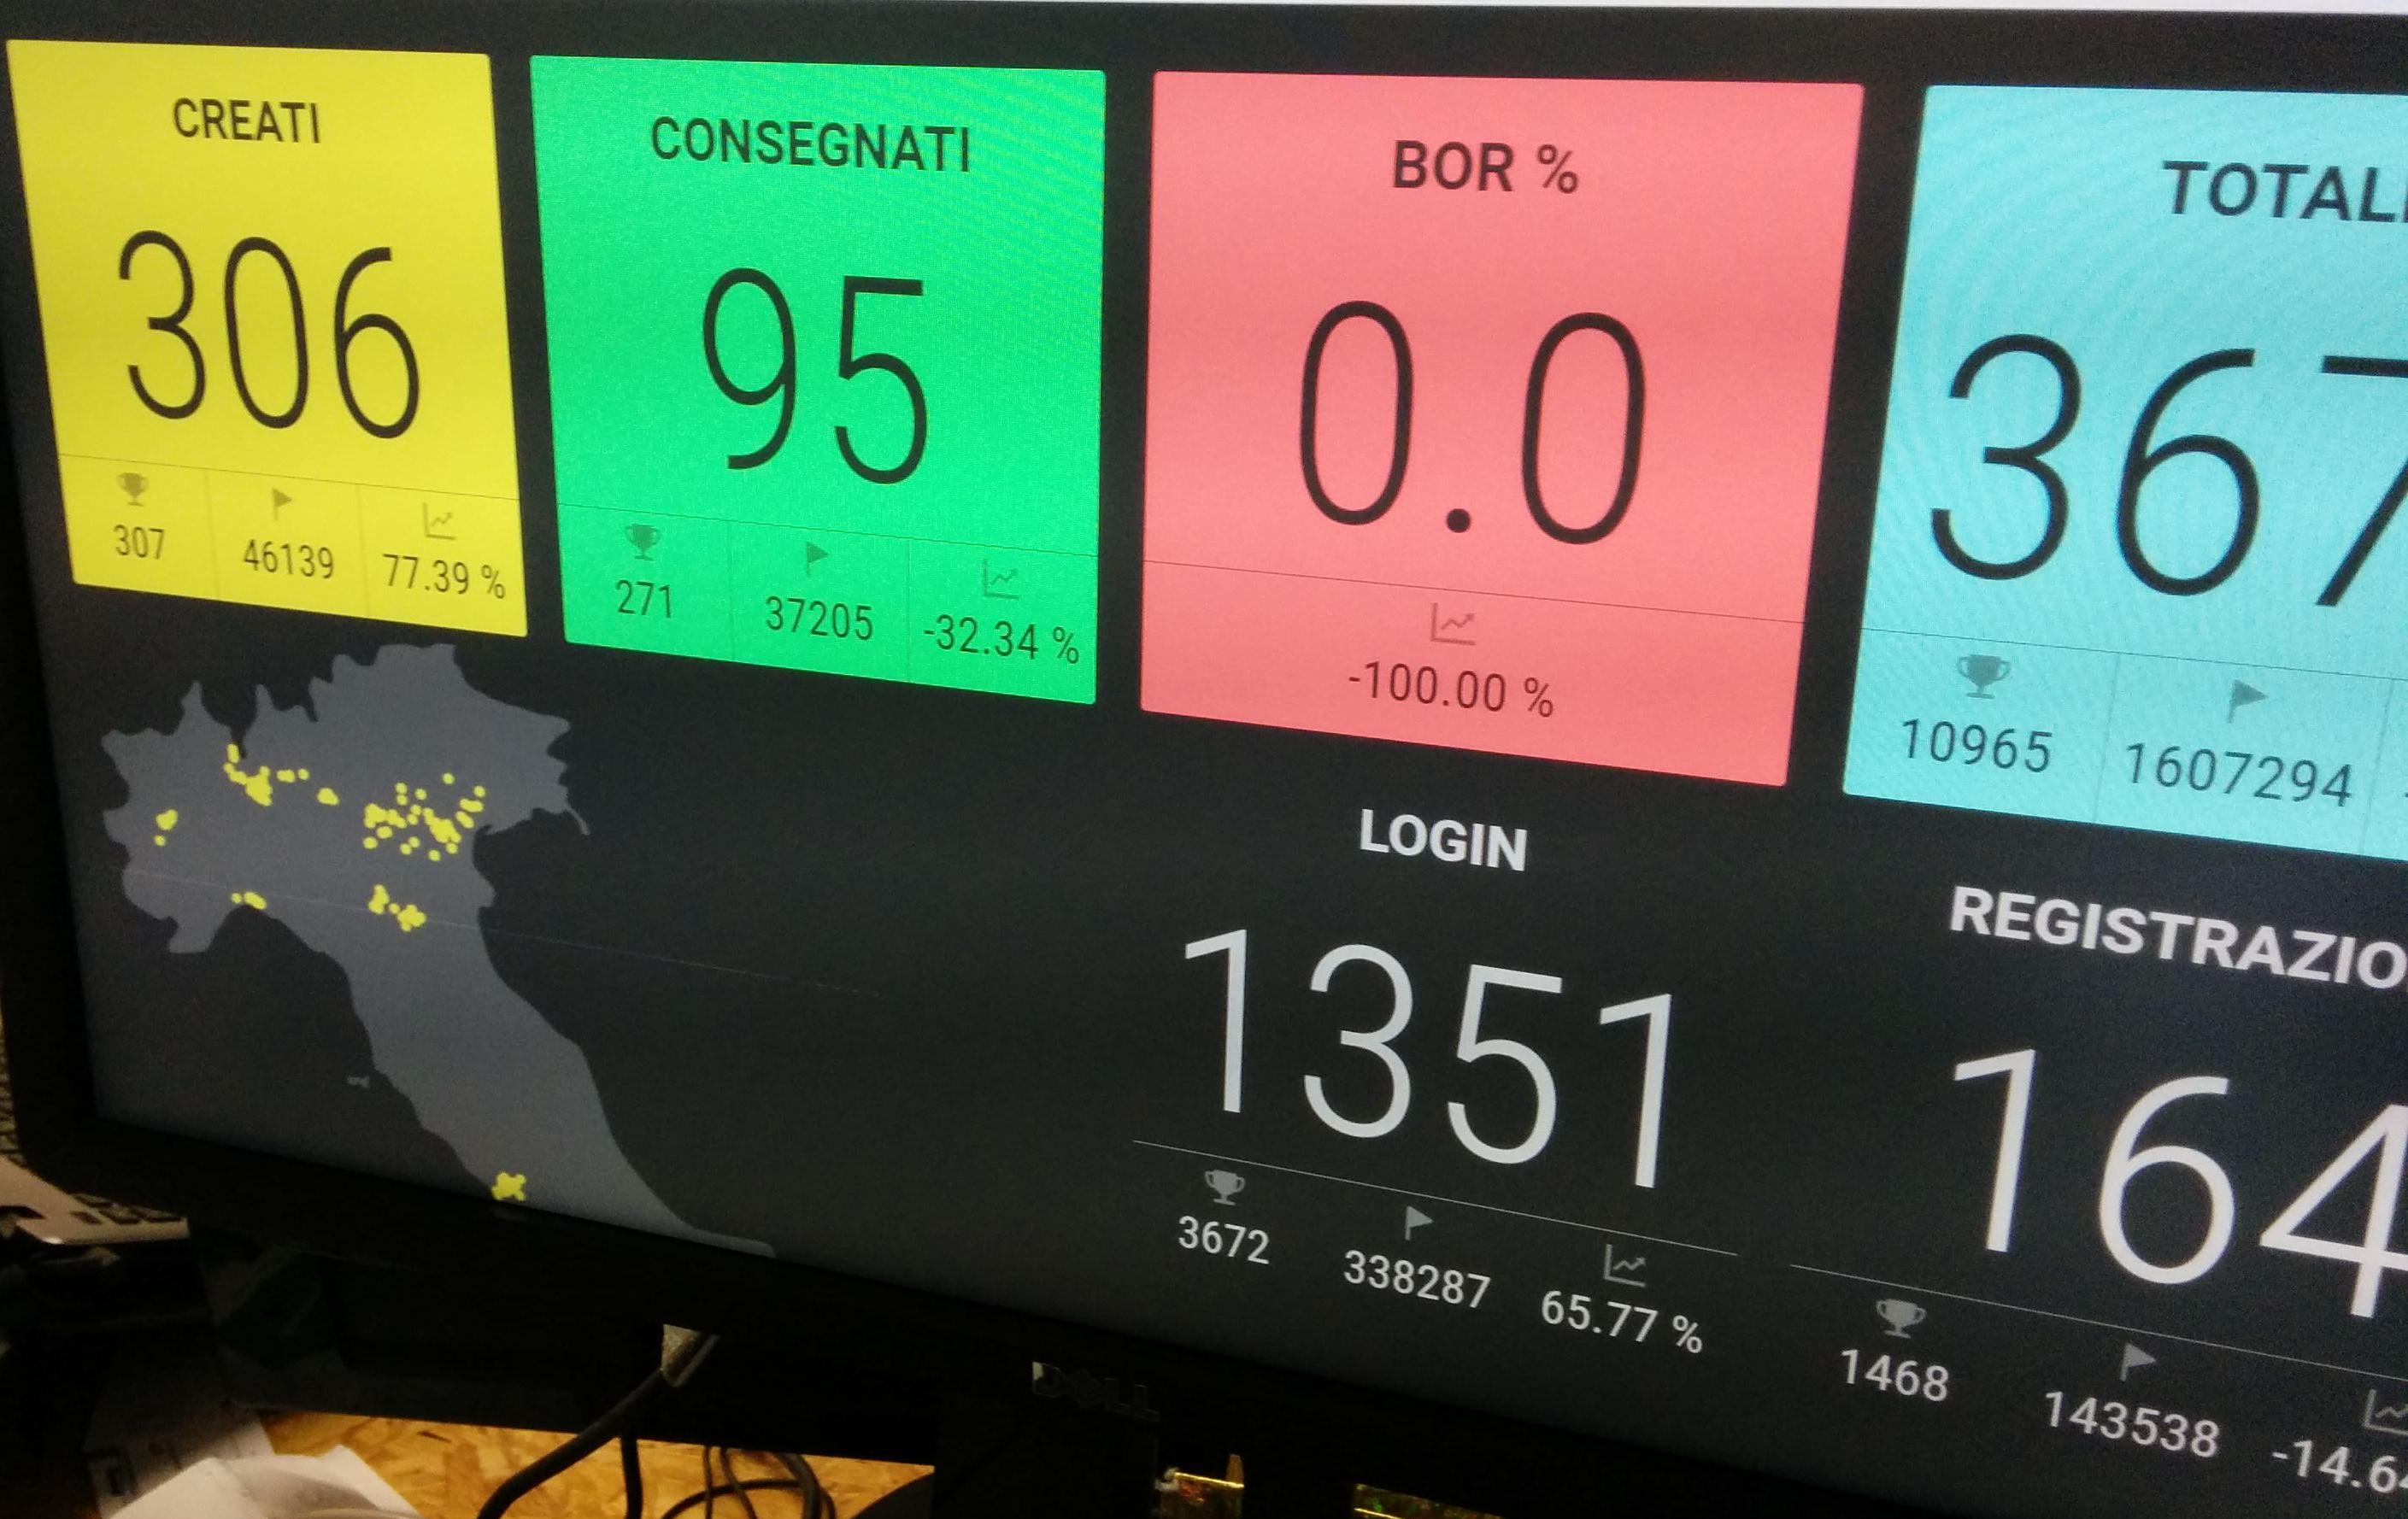
\includegraphics[width=0.95\linewidth, keepaspectratio]{socksberry_view}
  \caption{Foto del progetto Socksberry completato e operativo}
  \label{fig:socksberryView}
\end{figure}

\subsection{Difficoltà affrontate}
\label{subsec:socksberryDifficolta}

Inizialmente la fase di bootstrap dell'applicativo era associata alla prima connessione da parte di un \textit{client} e isolata da altri interlocutori.
Quindi per ogni \textit{client} connesso veniva effettuata una query iniziale e una \textit{subscription} dei \textit{topics} all'interno dello \textit{scope} del socket.
Si è poi reso necessario condividere questo modello tra tutti i socket, migliorando le performance e diminuendo il carico complessivo.

La comunicazione asincrona creata tramite \verb+WebSocket+ viene utilizzata prevalentemente in un'unica direzione: dal \textit{controller} verso la \textit{view}.
È stata proposta l'adozione dei \verb+SSE+, ma le notifiche non venivano inviate in tempo utile derivato dal delay progettuale.

La connessione da parte di un \textit{client} tramite \verb+WebSocket+ potrebbe venire effettuata mentre il \textit{controller} è in ancora in fase di bootstrap non ricevendo alcun dato e rimanendo inutilmente in attesa.
Abbiamo previsto, quindi, una fase ``init'' anche per la \textit{view}, aspettando la fase utile di scambio dati e attivando la grafica della \textit{dashboard} asincronamente.

\subsection{Conclusioni}
\label{subsec:socksberryConclusioni}

Si è scelto di non utilizzare il protocollo \verb+MQTT+ tra il \textit{controller} e la \textit{view} perché:
\begin{itemize}
  \item la batteria non è un fattore critico
  \item la banda non è un fattore critico
  \item la potenza computazionale non era condivisa con risorse critiche
  \item trattandosi di uno strumento di controllo interno non erano necessarie ottimizzazioni
\end{itemize}

      \section{SmIoT}
        \label{sec:smiot}
        Nella precedente sezione \ref{subsec:supermercato24StrutturaDatabase} è emersa la necessità di notificare a tutti i dispositivi connessi ogni azione intrapresa da un cliente in tempo reale.
Lo scopo di questo lavoro è valutare la migliore implementazione disponibile e compatibile con lo stack attuale.
Questo progetto è stato rinominato ``SmIoT'' dall'unione di ``Supermercato'' e ``IoT''.

\subsection{Analisi iniziale}
\label{subsec:smiotAnalisi}

\noindent
I requisiti iniziali sono:
\begin{itemize}
  \item sincronizzazione inserimento/modifica/eliminazione di un prodotto nel carrello
  \item notificare inserimento/eliminazione di un prodotto preferito
  \item notificare la transazione dello stato dell'ordine
  \item sincronizzare gli slot orari di ogni supermercato
\end{itemize}

\bigskip
\noindent
I possibili sviluppi dall'implementazione potrebbero essere:
\begin{itemize}
  \item creazione di una chat per l'assistenza clienti
  \item utilizzare notifiche push a fini di marketing
  \item fornire informazioni dettagliate sull'arrivo del fattorino
  \item analizzare i clienti connessi in tempo reale
\end{itemize}

Tutti i valori sono associati per utente e devono essere isolati ai suoi dispositivi.
L'utilizzo del servizio da parte dei dispositivi mobile, condiviso tra app e sito responsive, si attesta sul 50\%, mentre gli ordini fatti solo da app sono circa il 30\%.
Con questi dati si è scelto di non sottovalutare le difficoltà della \verb+UX+ dei \textit{client} non desktop.

\subsection{Implementazione}
\label{subsec:smiotImplementazione}

Attualmente tutti i requisiti sono gestiti tramite chiamate \verb+RESTful+ descritte nella sezione \ref{subsec:supermercato24StrutturaArchitettura}.
Il cambio di paradigma, verso una tipologia asincrona, dovrebbe migliorare l'esperienza generale del cliente aumentando la soddisfazione.

Grazie all'esperienza maturata con il precedente progetto della sezione \ref{sec:socksberry}, inizialmente era stato considerato l'utilizzo del \verb+WebSocket+.
Il primo mockup, infatti, utilizzava un'implementazione simile, ma i risultati, soprattutto verso i dispositivi smart, non erano abbastanza soddisfacenti.
La possibile degradazione della banda e il sovraccarico delle connessioni non garantivano la scalabilità e la qualità prevista inizialmente.

Si è dovuto cercare un protocollo alternativo che potesse garantire la stabilità necessaria per questi dispositivi.
Sono stati analizzati diversi protocolli quali: \verb+AMQP+, \verb+STOMP+ e \verb+MQTT+.
Il protocollo \verb+MQTT+, descritto nella sezione \ref{sec:mqtt}, teoricamente poteva soddisfare i requisiti iniziali.

È stato sviluppato un applicativo \verb+NodeJs+  (\textit{``broker''}) sul \textit{server} di produzione connesso con il KeyValue tramite una comunicazione \textit{publish}/\textit{subscribe} per ricevere gli aggiornamenti di ogni utente.
Il programma è riportato in appendice \ref{app:smiot_controller}.

Ogni \textit{client} una volta connesso e autenticato al sito, effettua l'\textit{handshake} verso il \textit{broker} tramite il \textit{token} di sessione che lo identifica all'interno del sistema.
Tramite protocollo \verb+MQTT+ viene concordato il giusto livello di \verb+QoS+ in base alla sua connessione.
Alla notifica di un evento, viene effettuato il \textit{dispatch} da parte del \textit{broker} all'utente appropriato, seguendo questo flow:
\begin{enumerate}
  \item connessione del dispositivo \textbf{A} del cliente Foo
  \item connessione del dispositivo \textbf{B} del cliente Foo
  \item connessione del dispositivo \textbf{C} del cliente Foo
  \item il dispositivo \textbf{A} aggiunge/modifica/elimina un prodotto/risorsa chiamata PUT/DELETE
  \item il controller Php effettua l'operazione del prodotto/risorsa e ``pubblica'' il relativo evento
  \item disconnessione del dispositivo \textbf{C} del cliente Foo
  \item il KeyValue consegna il messaggio al broker
  \item il broker spedisce il messaggio al dispositivo \textbf{B}
  \item il dispositivo \textbf{B} conferma il messaggio ed aggiorna le proprie risorse
\end{enumerate}

\begin{figure}[H]
  \centering
  \includegraphics[width=0.95\linewidth, keepaspectratio]{smiot_uml}
  \caption{Modello delle connessioni del progetto SmIoT}
  \label{fig:smiotUml}
\end{figure}

La possibilità di riutilizzare la stessa connessione \verb+MQTT+ per incapsulare le chiamate \verb+RESTful+ è ancora in fase embrionale.
Con questa possibilità si potrebbe sfruttare la comunicazione già instaurata invece di crearne una nuova per intraprendere l'azione.

\subsection{Difficoltà affrontate}
\label{subsec:smiotDifficolta}

Data la complessità dell'operazione, la migrazione è attualmente in fase di test; controllando la compatibilità con tutti i dispositivi.
Per evitare problemi di regressione, il modello dati non è stato variato completamente, permettendo di ripristinare le vecchie funzionalità dinamicamente.

Non è ancora possibile cambiare il \verb+QoS+ una volta connesso: il passaggio dal \verb+Wi-Fi+ al \verb+3G+ non fa aumentare il livello di qualità del servizio.
Si è scelto di effettuare nuovamente la connessione negoziando la qualità del servizio corretta.

Grazie ai ping \textit{KeepAlive} inviati dai vari dispositivi si possono interrompere le connessioni in esubero o fallite.

Attualmente l'1\% degli ordini mensili viene confermato in contemporanea tra due o più dispositivi e solo il primo viene confermato.
Si è scelto di applicare un \textit{mutex} alla risorsa condivisa ``carrello'' e lanciare un errore al tentativo di creazione contemporanea.
La sincronizzazione di questi così poco influenti non è stata ritenuta necessaria.

\subsection{Conclusioni}
\label{subsec:smiotConclusioni}

Dall'analisi dei dati, risulta che circa il 10\% degli ordini viene effettuato con una combinazione di più dispositivi.
Alcuni esempi potrebbero essere:
\begin{itemize}
  \item creazione della spesa durante il lavoro e relativa conferma dell'ordine a casa
  \item apertura dell'e-mail ``conferma account'' dal browser a seguito di una registrazione tramite app
  \item apertura delle e-mail \verb+CRM+ (\textit{Customer relationship management}) dal browser
\end{itemize}

Sincronizzando i dati tra questi \textit{device} non è più necessario, da parte dell'utente, ricaricare il proprio applicativo per notare le modifiche, diminuendo anche le chiamate verso il \textit{server}.
Inoltre l'introduzione graduale di queste feature, grazie al protocollo appropriato, non comporta nessun degrado della qualità dell'esperienza utente.

      \section{Analisi Competitor}
        \label{sec:competitor}
        Durante la fase progettuale sono stati analizzati i rispettivi competitor e altri servizi simili per osservare come hanno affrontato e risolto questo problema.

Recentemente, gli sviluppatori della chat Messanger di Facebook, per salvaguardare il consumo della batteria e ridurre le latenza dei messaggi, hanno iniziato a migrare il loro codebase verso il protocollo \verb+MQTT+ \cite{Facebook}.
Noti fornitori di servizi enterprise, quali AWS e IBM, hanno già sviluppato software \textit{ad hoc} basati su questo protocollo \cite{Ibm, Aws}.

Amazon ha preferito rimanere al protocollo \verb+HTTP+ e tramite chiamate \verb+AJAX+ asincrone, propaga le operazioni sul carrello.

Al contrario, Instacart, fornitore di servizi in stile Supermercato24, ha scelto di utilizzare il \verb+WebSocket+ come principale metodo di sincronizzazione dati.
Usando il servizio Firebase (acquistato da Google), riesce ad esternalizzare questo task, mantenendo il carrello aggiornato \cite{Instacart}.
Firebase è un servizio \verb+SaaS+ (\textit(Software as a service)) che permette il salvataggio e la sincronizzazione dei dati verso \textit{client} multipli.
Attraverso \verb+WebSocket+ propaga la risorsa aggiornata ad ogni cambiamento.

Si è ipotizzato che la differenza dell'implementazione tra Amazon e Instacart (e quindi Supermercato24) sia dovuto all'utilizzo medio delle due piattaforme da parte della clientela.
Se su Amazon il carrello si attesta su pochi \verb+SKU+ (\textit{Stock Keeping Unit}) e quindi con un minor tempo d'acquisto, per gli e-commerce di categoria \textit{food-and-drinks} gli \verb+SKU+ sono mediamente maggiori, con conseguente aumento del tempo necessario per concludere l'ordine \cite{InstacartAnalysis}.
Se su Supermercato24 il tempo medio di completamento di un ordine è di 40 minuti, è dunque necessario sincronizzare tempestivamente il carrello per poterlo concludere successivamente senza perdere dati tra i dispositivi.


  \newpage
  \thispagestyle{empty}
  \mbox{}

  \chapter{Valutazione sperimentale}
    \label{ch:evaluation}
    \lettrine{D}{i} seguito verranno confrontate le soluzioni proposte per mantenere i dati sincronizzati.
Nonostante la differenza del protocollo usato, entrambe condividono la stessa architettura sottostante e lo stesso pattern asincrono.

Verranno usati due approcci per validare la giusta implementazione.
Il primo approccio sarà quantitativo: in base al numero di messaggi inviati/ricevuti si confronteranno il consumo delle risorse e la capacità massima di invio/ricezione.
Il secondo approccio sarà qualitativo: verranno analizzati i pacchetti inviati/ricevuti descrivendo la sintassi di ognuno.

      \section{Confronto quantitativo}
        \label{sec:comparison}
        Si è analizzato il consumo medio di risorse in un dispositivo \verb+Android+ in diversi ambienti e la velocità di ricezione dei messaggi \cite{PowerProfiling}.

\bigskip
\noindent
Si sono usate le seguenti specifiche:
\begin{itemize}
\item cellulare modello Nexus 5 con \verb+Android 6+ completamente carico
\item analisi dettagliata del dispositivo tramite software \textit{adb} e \textit{Battery Historian} \cite{Adb, BatteryHistorian}
\item connessioni senza compressione e senza cifratura
\item \textit{back-end} installato localmente emulando i dati di produzione
\item libreria Socket.io@1.7.2 per il protocollo \verb+HTTP+
\item libreria Mqtt@3.1.1 per il protocollo \verb+MQTT+
\end{itemize}

\bigskip
\noindent
Il flow seguito è il seguente:
\begin{enumerate}
\item collegamento del cellulare tramite cavo USB con la modalità sviluppatore attivata
\item attivazione del demone di debugging \verb+./adb devices;+
\item eliminazione dei precedenti dump
  \begin{itemize}
  \item \verb+./adb shell dumpsys procstats --reset;+
  \item \verb+./adb shell dumpsys batterystats --reset;+
  \end{itemize}
\label{itm:comparisonDump}
\item lancio di 1024 benchmark in base al protocollo e alla funzionalità testata
\item download del dump \verb+./adb bugreport > bugreport.txt;+
\item analisi del dump tramite \textit{Battery Historian} con applicativo \textit{Docker}
\label{itm:comparisonHistorian}
\item ripetizione degli step \ref{itm:comparisonDump}-\ref{itm:comparisonHistorian} per 10 campioni
\item chiusa della modalità debug \verb+./adb kill-server;+
\end{enumerate}

\bigskip
\noindent
Le principali metriche osservate in ordine d'importanza sono:
\begin{description}
  \item[consumo della batteria] come requisito progettuale e principale indicatore della bontà sviluppata
  \item[bandwidth] utilizzato, per garantire un maggior traffico dati
  \item[CPU lato applicativo] per controllare l'utilizzo del protocollo da parte dell'applicazione
  \item[CPU lato sistema] per controllare le \textit{system calls} necessarie a mantenere la connessione
\end{description}

\bigskip
\noindent
Mentre si è deciso di omettere:
\begin{description}
  \item[tempo in foreground] dato che la sincronizzazione utilizza \textit{subroutine}
  \item[CPU lato applicativo] del \textit{server}, a favore della performance dei \textit{client}
  \item[latenza dei messaggi] poiché dai primi esami risultava trascurabile
\end{description}

\subsection{Creazione della connessione}
\label{sub:comparisonCreazione}

Si è iniziato ad osservare il costo della connessione iniziale con entrambi i protocolli.
Verrà analizzato il consumo di batteria medio per l'instaurazione della comunicazione.

\begin{itemize}
\item \verb+MQTT+ invia una serie di parametri iniziali quali: \textit{ClientId}, versione del protocollo, eventuale \textit{payload} di autenticazione e il metodo di \verb+QoS+ proposto dal client
\item \verb+HTTP+ invia una serie di headers opzionali per identificare correttamente la risorsa che si vuole ottenere. Utilizzando la porta \verb+HTTP+, viene effettuata una richiesta \textit{Upgrade} per effettuare uno switch del protocollo
\end{itemize}

Nella sezione \ref{sub:packetCreazione} è possibile notare nel dettaglio l'invio di questi pacchetti.
Si è analizzato la percentuale di batteria consumata, velocità dati e uso delle risorse in rapporto a un'ora di utilizzo \verb+Wi-Fi+.
Nell'appendice \ref{app:charCreazione} sono apprezzabili i grafici di questi test.

\begin{table}[H]
  \begin{center}
  \begin{tabular}{| c | l | l | l | l |}
    \hline
     & HTTP & deviazione std & MQTT & deviazione std \\ \hline
    \% utilizzo batteria / ora & \textbf{1.55} & 0.08 & 1.70 & 0.09 \\ \hline
    KBs / ora & \textbf{26649.28} & 2702.90 & 10770.50 & 1263.60 \\ \hline
    User CPU time / ora & 8.62 & 0.27 & \textbf{7.00} & 0.55 \\ \hline
    System CPU time / ora & 3.45 & 0.23 & \textbf{2.41} & 0.18 \\ \hline
  \end{tabular}
  \label{tab:comparisonCreazione2}
  \caption{Metriche osservate in un'ora di tentativi di connessione}
  \end{center}
\end{table}

La tabella mostra come l'iniziale richiesta tramite \verb+HTTP+ consumi meno risorse, data la ridotta quantità di dati inviata.
Poiché \verb+MQTT+ si fa carico di effettuare da subito la sottoscrizione ai \textit{topic} necessari, richiede due risposte dal parte del server.
Nel dettaglio, i pacchetti \ref{sub:packetCreazione} e \ref{sub:packetSottoscrizione} sono sequenziali.
\verb+MQTT+ conferma la \textit{subscription} ad ogni riconnessione tramite il flag \textit{cleanstart=true}, così facendo sono sempre necessarie due richieste per connessione, ciò depone a favore del protocollo \verb+HTTP+.
Disabilitando questa opzione si possono ottenere dei risultati simili per entrambi i protocolli, ma il \textit{server} dovrebbe salvarsi questa \textit{subscription} per un tempo determinato a priori.

\subsection{Mantenimento della connessione}
\label{sub:comparisonMantenimento}

Stabilire tempestivamente se la connessione verso il \textit{server} (e viceversa) è ancora disponibile, senza aspettare un lungo timeout \verb+TCP/IP+, aumenta le probabilità che il successivo pacchetto dati venga spedito (o ricevuto) e in caso negativo, è compito del \textit{client} cercare di ristabilire la comunicazione.

\begin{itemize}
\item \verb+MQTT+ fornisce nativamente il metodo \verb+PINGREQ+ che invia un ping per sapere se la connessione è ancora valida
\item \verb+HTTP+ non propone questa funzionalità, ma può essere integrata programmaticamente tramite un meccanismo di \textit{polling}
\end{itemize}

Sono stati effettuati diversi test per ogni timeout con un campione di dieci minuti.

\begin{table}[H]
  \begin{center}
  \begin{tabular}{| c | l | l | l | l |}
    \hline
     & \multicolumn{4}{|c|}{\% utilizzo batteria / ora} \\ \cline{2-5}
     & \multicolumn{2}{|c|}{3G} & \multicolumn{2}{|c|}{Wi-FI} \\ \hline
    intervallo secondi \textit{KeepAlive} & HTTP & MQTT & HTTP & MQTT \\ \hline
    60  & 1.11368 & \textbf{0.72280} & 0.15778 & \textbf{0.00994} \\ \hline
    120 & 0.48512 & \textbf{0.31856} & 0.08713 & \textbf{0.00417} \\ \hline
    240 & 0.33092 & \textbf{0.15842} & 0.02836 & \textbf{0.00169} \\ \hline
    480 & 0.08078 & \textbf{0.07806} & 0.00763 & \textbf{0.00051} \\ \hline
  \end{tabular}
  \label{tab:comparisonMantenimento}
  \caption{Consumo della batteria in entrambi gli ambienti per mantenere la connessione}
  \end{center}
\end{table}

Il ping nativo \ref{sub:packetMantenimento} \verb+MQTT+ è più conveniente in entrambi gli ambienti rispetto all'emulazione programmatica tramite \textit{pooling}.
Normalmente il costo della creazione della connessione è trascurabile, ma non il suo mantenimento nel tempo.
Se si considera che il 50\% di traffico proviene da mobile e che ci vogliono 40 minuti per completare un ordine, con un timeout di 240 secondi si riesce a risparmiare il 48\% di batteria per ordine rispetto al protocollo \verb+HTTP+.

\subsection{Ricezione dati}
\label{sub:comparisonRicezione}

La ricezione dei dati da parte dei \textit{client}, a seguito di un evento, è il principale utilizzo di questo pattern.
I messaggi dovrebbero essere recapitati, indipendentemente dalla qualità e dalla congestione della linea.

Sono stati inviati 1024 messaggi (1 byte ciascuno) il più velocemente possibile da parte del \textit{broker}.
È stato abilitato il flag \verb+QoS 1+, inibiti i ping \textit{KeepAlive} e si deliberatamente degradato la rete con un elevato rumore da parte di altri software installati.

\begin{table}[H]
  \begin{center}
  \begin{tabular}{| c | l | l | l | l |}
    \hline
     & \multicolumn{2}{|c|}{3G} & \multicolumn{2}{|c|}{Wi-FI} \\ \cline{2-5}
     & HTTP & MQTT & HTTP & MQTT \\ \hline
    messaggi / ora & 1462 & \textbf{160032} & 3382 & \textbf{263068} \\ \hline
    messaggi ricevuti & 237 / 1024 & \textbf{1024 / 1024} & 521 / 1024 & \textbf{1024 / 1024} \\ \hline
  \end{tabular}
  \label{tab:comparisonRicezione}
  \caption{Numero di messaggi ricevuti da parte del client}
  \end{center}
\end{table}

Grazie al \verb+QoS+ nativo \verb+MQTT+, si fa carico di controllare che tutti i messaggi siano effettivamente recapitati.
Data la criticità nella sincronizzazione dei dati, l'affidabilità della ricezione è un requisito iniziale.
Se un messaggio non è stato ricevuto, viene rispedito dal \textit{server} il prima possibile.

Non è stato previsto nessun meccanismo di \textit{queue} per discriminare se un messaggio è in ritardo, analizzando solo l'attendibilità dell'implementazione.
Si potrebbe aggiungere un identificativo incrementale per ogni risorsa scambiata e scartare gli aggiornamenti obsoleti.

Si è analizzato la percentuale di batteria consumata, velocità dati e uso delle risorse in rapporto a un'ora di utilizzo \verb+Wi-Fi+.
Nell'appendice \ref{app:charRicezione} sono apprezzabili i grafici di questi test.

\begin{table}[H]
  \begin{center}
  \begin{tabular}{| c | l | l | l | l |}
    \hline
     & HTTP & deviazione std & MQTT & deviazione std \\ \hline
    \% utilizzo batteria / ora & 4.12 & 0.25 & \textbf{1.11} & 0.31 \\ \hline
    KBs / ora & 15777.10 & 1888.67 & \textbf{23333.21} & 2720.71 \\ \hline
    User CPU time / ora & 21.17 & 1.56 & \textbf{3.72} & 0.79 \\ \hline
    System CPU time / ora & 3.33 & 0.17 & \textbf{2.46} & 0.45 \\ \hline
  \end{tabular}
  \label{tab:comparisonRicezione2}
  \caption{Metriche osservate in un'ora di ricezione dati}
  \end{center}
\end{table}

Dalla tabella si può evincere la leggerezza del protocollo \verb+MQTT+ confrontando il tempo speso da parte della \verb+CPU+ nello stato dell'applicazione.
Nello specifico è stato adottato la stessa codifica \textit{application/json; charset=utf-8} osservabile nella sezione \ref{sub:packetRicezione}.

      \section{Analisi pacchetti}
        \label{sec:packet}
        Tramite software \textit{Wireshark} si è analizzato i principali pacchetti scambiati, mostrando prima il pacchetto \verb+HTTP+ e poi \verb+MQTT+.

\bigskip
\noindent
Si sono usate le seguenti specifiche:
\begin{itemize}
\item analisi dettagliata dei pacchetti tramite software \textit{Wireshark}
\item connessioni senza compressione e senza cifratura
\item \textit{back-end} installato localmente emulando i dati di produzione
\end{itemize}

\subsection{Creazione della connessione}
\label{sub:packetCreazione}

Tramite protocollo \verb+HTTP+ viene effettuato l'\textit{handshake} necessario per creare il \textit{WebSocket}.
Tra l'indirizzo \textit{0x0040} e \textit{0x0070} si può notare il cambio di protocollo, come evidenziato nella sezione \ref{subsec:httpWebsocket}.
\verb+MQTT+ fornisce tutti i parametri necessari, si noti il token di sessione per autenticare la richiesta nel byte all'indirizzo \textit{0x0060}.

\begin{lstlisting}[language=bash, label={lst:packetCreazioneHttp}, captionpos=b, caption={HTTP Upgrade Request per creare il socket WS}, basicstyle=\scriptsize\ttfamily]
0000   02 00 00 00 45 00 00 e3 3e f2 40 00 40 06 00 00  ....E...>.@.@...
0010   7f 00 00 01 7f 00 00 01 0b b8 dc 7f 01 d3 94 ac  ................
0020   8d de 93 69 80 18 31 c3 fe d7 00 00 01 01 08 0a  ...i..1.........
0030   33 3c a5 2b 33 3c a5 2a 48 54 54 50 2f 31 2e 31  3<.+3<.*HTTP/1.1
0040   20 31 30 31 20 53 77 69 74 63 68 69 6e 67 20 50   101 Switching P
0050   72 6f 74 6f 63 6f 6c 73 0d 0a 55 70 67 72 61 64  rotocols..Upgrad
0060   65 3a 20 77 65 62 73 6f 63 6b 65 74 0d 0a 43 6f  e: websocket..Co
0070   6e 6e 65 63 74 69 6f 6e 3a 20 55 70 67 72 61 64  nnection: Upgrad
0080   65 0d 0a 53 65 63 2d 57 65 62 53 6f 63 6b 65 74  e..Sec-WebSocket
0090   2d 41 63 63 65 70 74 3a 20 66 63 72 6f 6f 2b 47  -Accept: fcroo+G
00a0   33 50 30 62 71 32 52 66 53 38 45 5a 39 6f 37 35  3P0bq2RfS8EZ9o75
00b0   72 6d 4b 45 3d 0d 0a 53 65 63 2d 57 65 62 53 6f  rmKE=..Sec-WebSo
00c0   63 6b 65 74 2d 45 78 74 65 6e 73 69 6f 6e 73 3a  cket-Extensions:
00d0   20 70 65 72 6d 65 73 73 61 67 65 2d 64 65 66 6c   permessage-defl
00e0   61 74 65 0d 0a 0d 0a                             ate....
\end{lstlisting}

\begin{lstlisting}[language=bash, label={lst:packetCreazioneMqtt}, captionpos=b, caption={MQTT Creazione socket}, basicstyle=\scriptsize\ttfamily]
0000   02 00 00 00 45 00 00 6c fe c2 40 00 40 06 00 00  ....E..l..@.@...
0010   7f 00 00 01 7f 00 00 01 de 5b 07 5b 56 1f e3 58  .........[.[V..X
0020   b5 ad d1 73 80 18 31 d7 fe 60 00 00 01 01 08 0a  ...s..1..`......
0030   33 65 87 64 33 65 87 62 10 36 00 04 4d 51 54 54  3e.d3e.b.6..MQTT
0040   04 c2 00 14 00 20 30 39 31 65 31 30 38 38 31 36  ..... 091e108816
0050   33 66 34 64 65 61 39 30 35 66 64 32 32 32 61 64  3f4dea905fd222ad
0060   34 61 66 36 61 66 00 06 66 6f 6f 62 61 72 00 00  4af6af..foobar..
\end{lstlisting}

\subsection{Sottoscrizione al topic}
\label{sub:packetSottoscrizione}

La sottoscrizione al topic \verb+HTTP+ viene effettuata in \verb+Javascript+ e viene spezzata in due richieste \verb+TCP+.
\verb+MQTT+ permette la sottoscrizione simultanea a più argomenti contemporaneamente con una singola richiesta.
Questo pacchetto viene inviato immediatamente dopo la creazione della connessione.
Il dettaglio dei pacchetti sono apprezzabili nell'appendice \ref{app:packetSottoscrizione}.

\subsection{Mantenimento della connessione}
\label{sub:packetMantenimento}

Il probe \textit{KeepAlive} in \verb+HTTP+ serve solo per controllare che la connessione sia ancora attiva, mentre \verb+MQTT+ si aspetta anche una risposta da parte il \textit{server}.

\begin{lstlisting}[language=bash, label={lst:packetMantenimentoHttq}, captionpos=b, caption={HTTP Probe KeepAlive}, basicstyle=\scriptsize\ttfamily]
0000   02 00 00 00 45 00 00 37 13 b4 40 00 40 06 00 00  ....E..7..@.@...
0010   7f 00 00 01 7f 00 00 01 0b b8 dc 7f 01 d3 98 5d  ...............]
0020   8d de 93 a7 80 18 31 c1 fe 2b 00 00 01 01 08 0a  ......1..+......
0030   33 3d 06 83 33 3d 06 83 81 01 33                 3=..3=....3
\end{lstlisting}

\begin{lstlisting}[language=bash, label={lst:packetMantenimentoMqtt}, captionpos=b, caption={MQTT Probe KeepAlive}, basicstyle=\scriptsize\ttfamily]
0000   02 00 00 00 45 00 00 36 26 3c 40 00 40 06 00 00  ....E..6&<@.@...
0010   7f 00 00 01 7f 00 00 01 de 5b 07 5b 56 1f e3 9c  .........[.[V...
0020   b5 ad d1 7c 80 18 31 d7 fe 2a 00 00 01 01 08 0a  ...|..1..*......
0030   33 65 e0 da 33 65 92 d7 c0 00                    3e..3e....
\end{lstlisting}

\subsection{Ricezione dati}
\label{sub:packetRicezione}

La serializzazione dei dati avviene attraverso il formato \verb+JSON+.
I dettagli dei pacchetti sono apprezzabili nell'appendice \ref{app:packetRicezione}.

\subsection{Chiusura della connessione}
\label{sub:packetChiusura}

Per entrambi i protocolli, la chiusura della connessione (senza interruzione forzata) viene semplicemente notificata al \textit{server}.

\begin{lstlisting}[language=bash, label={lst:packetChiusuraHtttp}, captionpos=b, caption={HTTP Chiusura della connessione}, basicstyle=\scriptsize\ttfamily]
0000   02 00 00 00 45 00 00 38 28 69 40 00 40 06 00 00  ....E..8(i@.@...
0010   7f 00 00 01 7f 00 00 01 0b b8 dc 7f 01 d3 99 54  ...............T
0020   8d de 93 c2 80 18 31 c1 fe 2c 00 00 01 01 08 0a  ......1..,......
0030   33 3d f1 42 33 3d f1 42 88 02 03 e9              3=.B3=.B....
\end{lstlisting}

\begin{lstlisting}[language=bash, label={lst:packetChiusuraMqtt}, captionpos=b, caption={MQTT Chiusura della connessione}, basicstyle=\scriptsize\ttfamily]
0000   02 00 00 00 45 00 00 36 8f 40 40 00 40 06 00 00  ....E..6.@@.@...
0010   7f 00 00 01 7f 00 00 01 de 5b 07 5b 56 1f e3 9e  .........[.[V...
0020   b5 ad d2 59 80 18 31 d0 fe 2a 00 00 01 01 08 0a  ...Y..1..*......
0030   33 65 f9 2a 33 65 eb 75 e0 00                    3e.*3e.u..
\end{lstlisting}


  \newpage
  \thispagestyle{empty}
  \mbox{}

  \chapter{Conclusioni}
    \label{ch:conclusion}
    \lettrine{S}{incronizzare} notevoli quantità di dati in tempo reale è un aspetto critico per molte piattaforme online.
L'utilizzo di una connessione persistente implica l'uso continuo della connessione dati, \textit{parsing} dello stream input e \textit{encoding} dello stream output.
Compiti non indifferenti a seguito della stima tra i 50 e 100 miliardi dei dispositivi connessi entro il 2020.
Fenomeni di \textit{spinlock} o di \textit{polling} per ottenere un risorsa aggiornata, dovrebbero essere abbandonati a favore di una comunicazione asincrona tra gli interlocutori.

Il lavoro di tesi si è sviluppato con un'introduzione ai paradigmi di comunicazione e background dei protocolli nel capitolo \ref{ch:background}.
Nel capitolo \ref{ch:solution} sono state proposte due soluzioni implementative diverse con una panoramica tecnica dei software attuali presso l'azienda Supermercato24.
Queste applicazioni sono state poi valutate tramite test nel capitolo \ref{ch:evaluation}.

Le prove effettuate hanno confermato come sia estremamente complesso costruire un modello che caratterizzi al meglio il risparmio di risorse nella creazione e nel mantenimento della connessione.
Tra queste variabili, di cui bisogna tenere necessariamente conto, c'è la reale possibilità che i pacchetti dati possano non arrivare a destinazione.
Di conseguenza la qualità del servizio deve essere una prerogativa irrinunciabile.

\verb+HTTP+, ampiamente utilizzato nella rete, nonostante sia avido di risorse garantisce un buon punto di partenza.
L'introduzione del \verb+WebSocket+ che implementa la comunicazione asincrona, ha permesso a questo protocollo di mantenersi ancora \textit{standard de facto} in Internet.
La nuova versione di questo protocollo aprirà le porte a nuovi scenari, come già sta facendo Google per la modifica dei documenti in tempo reale in \textit{Drive}.

\verb+MQTT+, di contro, è stato progettato per soddisfare da subito queste esigenze offrendo una serie di metodi nativi sgravando lo sviluppatore da questo compito.
La garanzia della consegna del messaggio prevista su tre livelli a secondo dalla criticità e la leggerezza dello stream dati, lo pone come un'alternativa più che valida.

Dalle verifiche sperimentali sono emerse le differenze tra i due protocolli sulle risorse utilizzate.
In un'ora di test il consumo di batteria con \verb+HTTP+ è il triplo rispetto a \verb+MQTT+.
Considerato il tempo trascorso dalla CPU eseguendo il codice nello \textit{user space}, denota la leggerezza del secondo protocollo.

Grazie a questa analisi è stato approvata la sperimentazione del protocollo \verb+MQTT+ come vettore nella sincronizzazione dati lato e-commerce.
Un altro problema attuale in Supermercato24 è il consumo significativo del gestionale dei fattorini.
La comunicazione della posizione geografica tramite chiamate \verb+AJAX+, esaurisce velocemente la batteria dei dispositivi; problema comune ad altri servizi simili come Deliveroo, Foodora e Just Eat.
L'utilizzo di \textit{power bank} a supporto diventa quindi indispensabile per poter affrontare più ordini.
Concluso con successo il test del progetto \ref{sec:smiot} verrà valutata in futuro questa migrazione.
Uno sviluppo interessante sarebbe confrontare questa possibile evoluzione ed i benefici ottenuti.
Un'altra opportunità potrebbe essere l'approfondimento di questi i test con l'attivazione della compressione e della crittografia, sacrificando la potenza computazionale a favore della connessione dati.

Concludendo, i protocolli proposti rappresentano soltanto un piccolo insieme.
L'affidabilità e la compatibilità restano gli ambiti in cui la ricerca dovrà muoversi in preparazione della crescita esponenziale nell'ambiente \verb+IoT+.


  \newpage
  \thispagestyle{empty}
  \mbox{}

  \appendix

  \chapter{Sorgenti}
    \section{Socksberry Controller}
      \label{app:socksberry_controller}
      \begin{lstlisting}[language=java, captionpos=b, caption={Doppio broker HTTP: KeyValue e WebSocket}, basicstyle=\scriptsize\ttfamily]
var nsp = io.of('/socksberry').use(function(socket, next) {

  next();
});

/*
 * pub/sub pattern
 */
nsp.on('connection', function(socket) {

  /*
   * subscribe
   */
  var sub = cached(my); // KeyValue broker

  /**
   * subscribe local object as broker topic as callback
   *
   * @param {String} name - model name
   * @param {Object} object - model object
   * @param {Integer} counter - switch between KeyValue Database
   */
  modelsLoop(function(name, object, counter) {

    sub.select(counter, function() {

      sub.subscribe(name);
    });
  });

  /**
   * message from KeyValue broker
   */
  sub.on('message', function(channel, message) {

    if (models[channel] === undefined) { // missing rigth channel
      return; // next
    }
    var cmd = JSON.parse(message);

    models[channel].update(cmd.event.split('.'), cmd.data,
      function(err, res) { // update local model

        if (res !== null) {

          var out = {
            status: true,
            data: res
          }; // stringify data, instead of send out directly
          nsp.to(socket.id).emit(channel, JSON.stringify(out));
        }
      });
  });

  /**
   * event from WebSocket broker
   */
  socket.on('disconnect', function() {

    /**
     * unsubscribe local object from broker topic as callback
     *
     * @param {String} name - model name
     */
    modelsLoop(function(name) {

      sub.unsubscribe(name);
    });
  }).on('init', function() {

    nsp.to(socket.id).emit('init', JSON.stringify(staticOut));
  });
});
\end{lstlisting}

    \section{Socksberry View}
      \label{app:socksberry_view}
      \begin{lstlisting}[language=java, captionpos=b, caption={HTTP WebSocket subscriber}, basicstyle=\scriptsize\ttfamily]
// define socket connection handler
var manager, socket;

// in case of network errors, init data with static (empty) model
app.setOfflineModel = function() {
  app.user = _data.user;
  app.s24 = _data.s24;
  app.offline = true;
};

// After manager has installed correctly the connection with server,
// init socket and initialize event callback
app.initSocket = function() {

  socket = manager.socket('/socksberry');

  // define socket io callback
  socket.on('error', function(data) {

    console.error(data);
    app.offline = true;

  }).on('disconnect', function() {

    console.log('disconnect');
    app.offline = true;

  }).on('connect', function() {

    console.log('connect');
    socket.emit('init');
    app.offline = true;
    app.placeholderMap = false;

  }).on('user', function(data) {

    app.user = JSON.parse(data).data;

  }).on('s24', function(data) {

    app.s24 = JSON.parse(data).data;

  }).on('init', function(data) {

    var data = JSON.parse(data).data;
    app.s24 = data.s24;
    app.user = data.user;
    app.offline = false;

  });
};

// init Socket IO
app.init = function() {

  var url = config.protocol + '://' + config.ip + ':' + config.port;
  var opts = {
    reconnectionDelay: 10000
  };
  manager = io.Manager(url, opts);
  // save reference, for debug purpose
  // window.manager = manager;

  // static (offline) initialization
  app.setOfflineModel();
  app.placeholderMap = true;
  // init socket
  app.initSocket();
};

// See https://github.com/Polymer/polymer/issues/1381
window.addEventListener('WebComponentsReady', function() {
  // imports are loaded and elements have been registered
  // init data
  app.init();
});
\end{lstlisting}

    \section{SmIoT Controller}
      \label{app:smiot_controller}
      \begin{lstlisting}[language=java, captionpos=b, caption={Dispatcher broker MQTT}, basicstyle=\scriptsize\ttfamily]
/**
 * move consumer outside from server.
 * Otherwise duplicated messages are sent from every client, using dispatcher
 */
consumerInterface.on('message_buffer', function(channel, message) {

  var channelString = channel.toString();
  var funnels = channelString.split('/');
  var userId = funnels[0];

  if (dispatcher.emit(userId, funnels.slice(1).join('/'), message)) { // had user
    // pass
  } else { // remove subscriber
    consumerInterface.unsubscribe(channelString);
  }
});

/**
 * transform net stream into mqtt client
 */
serverInterface.on('connection', function(stream) {

  stream.setKeepAlive(options.keepAlive);
  stream.setNoDelay(options.noDelay);
  stream.setTimeout(options.timeout);
  var client = mqttConnection(stream);

  /**
   * connection between broker interface and server interface
   *
   * @function publisher
   * @param {Buffer} channel - client topic
   * @param {Buffer} message - client message
   * @param {Boolean} [pingreq] - check if this eventListener is alive
   */
  var publisher = function(channel, message, pingreq) {

    if (pingreq) {
      return;
    }

    if (client.authorized && client.topics[client.topicPrefix + channel]) {
      client.publish({
        qos: returnCode.SUBSCRIPTION_QOS_0,
        topic: channel,
        payload: message
      });
    }
  };

  client.once('connect', function(packet) {

    /**
     * <pre>
     * `version`: the protocol version string
     * `versionNum`: the protocol version number
     * `keepalive`: the client's keepalive period
     * `clientId`: the client's ID
     * `will`: an object with the following keys:
     *   `topic`: the client's will topic
     *   `payload`: the will message
     *   `retain`: will retain flag
     *   `qos`: will qos level
     * `clean`: clean start flag
     * `username`: v3.1 username
     * `password`: v3.1 password
     * </pre>
     */
    stream.pause(); // pauses the reading of data

    var response = {
      returnCode: returnCode.CONNECTION_REFUSED_SERVER_UNAVAILABLE
    };

    var userToken = packet.username;
    if (!userToken) {
      response.returnCode = returnCode.CONNECTION_REFUSED_NOT_AUTHORIZED;
      stream.resume();
      client.connack(response);
      return;
    }

    brokerInterface.get(userToken, function(err, userId) {

      if (err) {
        // pass
      } else if (userId) { // client init

        dispatcher.on(userId, publisher);

        client.authorized = true;
        client.topics = {};
        client.clientId = packet.clientId;
        client.userId = userId;
        client.userToken = userToken;
        client.topicPrefix = userId + '/';

        response.returnCode = returnCode.CONNECTION_ACCEPTED;
      } else {
        response.returnCode = returnCode.CONNECTION_REFUSED_BAD_CREDENTIALS;
      }

      stream.resume();
      client.connack(response);
    });
  }).on('subscribe', function(packet) {

    var response = {
      messageId: packet.messageId,
      granted: []
    };

    var channels = [];
    var notGranted = [];
    var subscriptions = {};
    for (var i = 0, ii = packet.subscriptions.length; i < ii; ++i) {
      var topic = packet.subscriptions[i].topic;
      notGranted[i] = returnCode.SUBSCRIPTION_FAILURE;

      if (client.authorized) {
        response.granted[i] = returnCode.SUBSCRIPTION_QOS_0;
        topic = client.topicPrefix + topic;

        if (subscriptions[topic] === undefined) { // unique
          subscriptions[topic] = true;
          channels[i] = topic;
        }
      }
    }

    if (client.authorized === false) {
      response.granted = notGranted;
      client.suback(response);
      return;
    }

    // https://github.com/NodeRedis/node_redis/issues/1188
    consumerInterface.subscribe(channels, function(err, latestChannel) {

      if (err) {
        response.granted = notGranted;
      } else if (latestChannel) {
        Object.assign(client.topics, subscriptions);
      } else {
        response.granted = notGranted;
      }
      client.suback(response);
    });
  }).on('unsubscribe', function(packet) {

    var response = {
      messageId: packet.messageId
    };

    if (!client.authorized) {
      client.unsuback(response);
      return;
    }

    var unsubscriptions = [];
    for (var i = 0, ii = packet.unsubscriptions.length; i < ii; ++i) {
      var topic = client.topicPrefix + packet.unsubscriptions[i];

      if (client.topics[topic]) {
        unsubscriptions.push(topic);
        delete (client.topics[topic]);
      }
    }

    client.unsuback(response);
  }).on('pingreq', function() {

    if (client.authorized) {
      client.pingresp();
    } else {
      client.destroy();
    }
  }).once('close', function() {

    if (client.stream.destroyed === false) {
      client.destroy();
    }

    if (!client.authorized) {
      return;
    }

    client.authorized = false;
    dispatcher.removeListener(client.userId, publisher);
    var unsubscriptions = Object.keys(client.topics);
    if (!unsubscriptions) {
      return; // pass
    }

    if (!dispatcher.emit(client.userId, [], true)) {
      consumerInterface.unsubscribe(unsubscriptions, function(err) {

        if (err) {
          // pass
        } else {
          client.topics = {};
        }
      });
    }
  }).once('disconnect', function() {

    client.destroy();
  }).once('error', function(err) {

    client.destroy();
  });

  stream.once('timeout', function() {

    client.destroy();
  });
});
\end{lstlisting}

  \chapter{Test}
    \section{Grafici risultati}
      \label{app:chart}
      \subsection{Creazione della connessione}
\label{app:charCreazione}

\begin{figure}[H]
  \centering
  \includegraphics[width=0.95\linewidth, keepaspectratio]{batteryc}
  \caption{\% utilizzo batteria / ora nella creazione della connessione}
  \label{fig:batteryc}
\end{figure}

\begin{figure}[H]
  \centering
  \includegraphics[width=0.95\linewidth, keepaspectratio]{kbc}
  \caption{KBs / ora nella creazione della connessione}
  \label{fig:kbc}
\end{figure}

\begin{figure}[H]
  \centering
  \includegraphics[width=0.95\linewidth, keepaspectratio]{cpuuc}
  \caption{User CPU time / ora nella creazione della connessione}
  \label{fig:cpuuc}
\end{figure}

\begin{figure}[H]
  \centering
  \includegraphics[width=0.95\linewidth, keepaspectratio]{cpusc}
  \caption{System CPU time / ora nella creazione della connessione}
  \label{fig:cpusc}
\end{figure}

\subsection{Ricezione dati}
\label{app:charRicezione}

\begin{figure}[H]
  \centering
  \includegraphics[width=0.95\linewidth, keepaspectratio]{batteryp}
  \caption{\% utilizzo batteria / ora nella ricezione dei dati}
  \label{fig:batteryp}
\end{figure}

\begin{figure}[H]
  \centering
  \includegraphics[width=0.95\linewidth, keepaspectratio]{kbp}
  \caption{KBs / ora nella ricezione dei dati}
  \label{fig:kbp}
\end{figure}

\begin{figure}[H]
  \centering
  \includegraphics[width=0.95\linewidth, keepaspectratio]{cpuup}
  \caption{User CPU time / ora nella ricezione dei dati}
  \label{fig:cpuup}
\end{figure}

\begin{figure}[H]
  \centering
  \includegraphics[width=0.95\linewidth, keepaspectratio]{cpusp}
  \caption{System CPU time / ora nella ricezione dei dati}
  \label{fig:cpusp}
\end{figure}

    \section{Dettaglio dei pacchetti}
      \label{app:hexdump}
      \subsection{Sottoscrizione al topic}
\label{app:packetSottoscrizione}

\begin{lstlisting}[language=bash, label={lst:packetSottoscrizioneHttq}, captionpos=b, caption={HTTP Sottoscrizione al topic "socksberry"}, basicstyle=\scriptsize\ttfamily]
0000   02 00 00 00 45 00 02 4b 1d 79 40 00 40 06 00 00  ....E..K.y@.@...
0010   7f 00 00 01 7f 00 00 01 dc 75 0b b8 47 fe 66 15  .........u..G.f.
0020   76 23 7f d6 80 18 31 3c 00 40 00 00 01 01 08 0a  v#....1<.@......
0030   33 3c a5 6d 33 3c a5 27 50 4f 53 54 20 2f 73 6f  3<.m3<.'POST /so
0040   63 6b 65 74 2e 69 6f 2f 3f 45 49 4f 3d 33 26 74  cket.io/?EIO=3&t
0050   72 61 6e 73 70 6f 72 74 3d 70 6f 6c 6c 69 6e 67  ransport=polling
0060   26 74 3d 4c 65 71 32 37 65 52 26 73 69 64 3d 58  &t=Leq27eR&sid=X
0070   64 74 62 59 78 68 6c 61 76 4c 6d 4d 51 71 51 41  dtbYxhlavLmMQqQA
0080   41 41 46 20 48 54 54 50 2f 31 2e 31 0d 0a 48 6f  AAF HTTP/1.1..Ho
0090   73 74 3a 20 31 32 37 2e 30 2e 30 2e 31 3a 33 30  st: 127.0.0.1:30
00a0   30 30 0d 0a 43 6f 6e 6e 65 63 74 69 6f 6e 3a 20  00..Connection:
00b0   6b 65 65 70 2d 61 6c 69 76 65 0d 0a 43 6f 6e 74  keep-alive..Cont
00c0   65 6e 74 2d 4c 65 6e 67 74 68 3a 20 31 36 0d 0a  ent-Length: 16..
00d0   41 63 63 65 70 74 3a 20 2a 2f 2a 0d 0a 4f 72 69  Accept: */*..Ori
00e0   67 69 6e 3a 20 68 74 74 70 3a 2f 2f 31 32 37 2e  gin: http://127.
00f0   30 2e 30 2e 31 3a 33 30 30 30 0d 0a 55 73 65 72  0.0.1:3000..User
0100   2d 41 67 65 6e 74 3a 20 4d 6f 7a 69 6c 6c 61 2f  -Agent: Mozilla/
0110   35 2e 30 20 28 4d 61 63 69 6e 74 6f 73 68 3b 20  5.0 (Macintosh;
0120   49 6e 74 65 6c 20 4d 61 63 20 4f 53 20 58 20 31  Intel Mac OS X 1
0130   30 5f 31 32 5f 33 29 20 41 70 70 6c 65 57 65 62  0_12_3) AppleWeb
0140   4b 69 74 2f 35 33 37 2e 33 36 20 28 4b 48 54 4d  Kit/537.36 (KHTM
0150   4c 2c 20 6c 69 6b 65 20 47 65 63 6b 6f 29 20 43  L, like Gecko) C
0160   68 72 6f 6d 65 2f 35 38 2e 30 2e 33 30 30 34 2e  hrome/58.0.3004.
0170   33 20 53 61 66 61 72 69 2f 35 33 37 2e 33 36 0d  3 Safari/537.36.
0180   0a 43 6f 6e 74 65 6e 74 2d 74 79 70 65 3a 20 74  .Content-type: t
0190   65 78 74 2f 70 6c 61 69 6e 3b 63 68 61 72 73 65  ext/plain;charse
01a0   74 3d 55 54 46 2d 38 0d 0a 44 4e 54 3a 20 31 0d  t=UTF-8..DNT: 1.
01b0   0a 52 65 66 65 72 65 72 3a 20 68 74 74 70 3a 2f  .Referer: http:/
01c0   2f 31 32 37 2e 30 2e 30 2e 31 3a 33 30 30 30 2f  /127.0.0.1:3000/
01d0   0d 0a 41 63 63 65 70 74 2d 45 6e 63 6f 64 69 6e  ..Accept-Encodin
01e0   67 3a 20 67 7a 69 70 2c 20 64 65 66 6c 61 74 65  g: gzip, deflate
01f0   2c 20 62 72 0d 0a 41 63 63 65 70 74 2d 4c 61 6e  , br..Accept-Lan
0200   67 75 61 67 65 3a 20 69 74 2d 49 54 2c 69 74 3b  guage: it-IT,it;
0210   71 3d 30 2e 38 2c 65 6e 2d 55 53 3b 71 3d 30 2e  q=0.8,en-US;q=0.
0220   36 2c 65 6e 3b 71 3d 30 2e 34 0d 0a 43 6f 6f 6b  6,en;q=0.4..Cook
0230   69 65 3a 20 69 6f 3d 58 64 74 62 59 78 68 6c 61  ie: io=XdtbYxhla
0240   76 4c 6d 4d 51 71 51 41 41 41 46 0d 0a 0d 0a     vLmMQqQAAAF....

0000   02 00 00 00 45 00 00 44 c6 90 40 00 40 06 00 00  ....E..D..@.@...
0010   7f 00 00 01 7f 00 00 01 dc 75 0b b8 47 fe 68 2c  .........u..G.h,
0020   76 23 7f d6 80 18 31 3c fe 38 00 00 01 01 08 0a  v#....1<.8......
0030   33 3c a5 6d 33 3c a5 27 31 33 3a 34 30 2f 73 6f  3<.m3<.'13:40/so
0040   63 6b 73 62 65 72 72 79                          cksberry
\end{lstlisting}

\begin{lstlisting}[language=bash, label={lst:packetSottoscrizioneMqtt}, captionpos=b, caption={MQTT Sottoscrizione al topic "smiot"}, basicstyle=\scriptsize\ttfamily]
0000   02 00 00 00 45 00 00 40 6c ed 40 00 40 06 00 00  ....E..@l.@.@...
0010   7f 00 00 01 7f 00 00 01 de 5b 07 5b 56 1f e3 90  .........[.[V...
0020   b5 ad d1 77 80 18 31 d7 fe 34 00 00 01 01 08 0a  ...w..1..4......
0030   33 65 92 d6 33 65 87 65 82 0a 00 01 00 05 73 6d  3e..3e.e......sm
0040   69 6f 74 00                                      iot.
\end{lstlisting}

\subsection{Ricezione dati}
\label{app:packetRicezione}

\begin{lstlisting}[label={lst:packetRicezioneHttp}, captionpos=b, caption={HTTP Payload dati inviato dal server}, basicstyle=\scriptsize\ttfamily]
0000   02 00 00 00 45 00 01 22 ba 6d 40 00 40 06 00 00  ....E..".m@.@...
0010   7f 00 00 01 7f 00 00 01 0b b8 dc 7f 01 d3 98 63  ...............c
0020   8d de 93 b0 80 18 31 c1 ff 16 00 00 01 01 08 0a  ......1.........
0030   33 3d b1 8c 33 3d 67 ec 81 7e 00 ea 34 32 2f 73  3=..3=g..~..42/s
0040   6f 63 6b 73 62 65 72 72 79 2c 5b 22 75 73 65 72  ocksberry,["user
0050   22 2c 22 7b 5c 22 73 74 61 74 75 73 5c 22 3a 74  ","{\"status\":t
0060   72 75 65 2c 5c 22 64 61 74 61 5c 22 3a 7b 5c 22  rue,\"data\":{\"
0070   72 65 67 69 73 74 72 61 74 69 6f 6e 5c 22 3a 7b  registration\":{
0080   5c 22 64 61 69 6c 79 5c 22 3a 30 2c 5c 22 64 61  \"daily\":0,\"da
0090   69 6c 79 5f 72 65 63 6f 72 64 5c 22 3a 31 35 39  ily_record\":159
00a0   2c 5c 22 74 6f 74 61 6c 5c 22 3a 33 31 37 2c 5c  ,\"total\":317,\
00b0   22 76 61 72 69 61 74 69 6f 6e 5c 22 3a 2d 31 30  "variation\":-10
00c0   30 7d 2c 5c 22 73 65 73 73 69 6f 6e 5c 22 3a 7b  0},\"session\":{
00d0   5c 22 64 61 69 6c 79 5c 22 3a 32 2c 5c 22 64 61  \"daily\":2,\"da
00e0   69 6c 79 5f 72 65 63 6f 72 64 5c 22 3a 31 31 38  ily_record\":118
00f0   33 2c 5c 22 74 6f 74 61 6c 5c 22 3a 32 35 39 35  3,\"total\":2595
0100   31 2c 5c 22 76 61 72 69 61 74 69 6f 6e 5c 22 3a  1,\"variation\":
0110   2d 39 38 2e 37 33 33 39 31 30 31 30 37 36 31 32  -98.733910107612
0120   33 7d 7d 7d 22 5d                                3}}}"]
\end{lstlisting}

\begin{lstlisting}[label={lst:packetRicezioneMqtt}, captionpos=b, caption={MQTT Payload dati inviato dal server}, basicstyle=\scriptsize\ttfamily]
0000   02 00 00 00 45 00 01 05 11 c0 40 00 40 06 00 00  ....E.....@.@...
0010   7f 00 00 01 7f 00 00 01 07 5b de 5b b5 ad d1 88  .........[.[....
0020   56 1f e3 9e 80 18 31 d5 fe f9 00 00 01 01 08 0a  V.....1.........
0030   33 65 eb 75 33 65 eb 75 7b 5c 22 73 74 61 74 75  3e.u3e.u{\"statu
0040   73 5c 22 3a 74 72 75 65 2c 5c 22 64 61 74 61 5c  s\":true,\"data\
0050   22 3a 7b 5c 22 72 65 67 69 73 74 72 61 74 69 6f  ":{\"registratio
0060   6e 5c 22 3a 7b 5c 22 64 61 69 6c 79 5c 22 3a 30  n\":{\"daily\":0
0070   2c 5c 22 64 61 69 6c 79 5f 72 65 63 6f 72 64 5c  ,\"daily_record\
0080   22 3a 31 35 39 2c 5c 22 74 6f 74 61 6c 5c 22 3a  ":159,\"total\":
0090   33 31 37 2c 5c 22 76 61 72 69 61 74 69 6f 6e 5c  317,\"variation\
00a0   22 3a 2d 31 30 30 7d 2c 5c 22 73 65 73 73 69 6f  ":-100},\"sessio
00b0   6e 5c 22 3a 7b 5c 22 64 61 69 6c 79 5c 22 3a 32  n\":{\"daily\":2
00c0   2c 5c 22 64 61 69 6c 79 5f 72 65 63 6f 72 64 5c  ,\"daily_record\
00d0   22 3a 31 31 38 33 2c 5c 22 74 6f 74 61 6c 5c 22  ":1183,\"total\"
00e0   3a 32 35 39 35 31 2c 5c 22 76 61 72 69 61 74 69  :25951,\"variati
00f0   6f 6e 5c 22 3a 2d 39 38 2e 37 33 33 39 31 30 31  on\":-98.7339101
0100   30 37 36 31 32 33 7d 7d 7d                       076123}}}
\end{lstlisting}


  \medskip
  \newrefcontext[sorting=none]
  \printbibliography[heading=bibintoc, title={Bibliografia}]

\end{document}
